\documentclass[a4paper,11pt,twoside,openright]{memoir}

% Castellano
\usepackage[spanish]{babel}
\selectlanguage{spanish}
\usepackage[utf8]{inputenc}
\usepackage{placeins}

\RequirePackage{booktabs}
\RequirePackage[table]{xcolor}
\RequirePackage{xtab}
\RequirePackage{multirow}

% Links
\usepackage[colorlinks]{hyperref}
\hypersetup{
	allcolors = {red}
}

% Ecuaciones
\usepackage{amsmath}

%Anotaciones TODO

\usepackage{todonotes}

%Color
\usepackage{color}
\definecolor{javapurple}{rgb}{0.5,0,0.35}
\definecolor{pgreen}{rgb}{0,0.5,0}
\definecolor{pred}{rgb}{0.9,0,0}
\definecolor{pgrey}{rgb}{0.46,0.45,0.48}

%Código
\usepackage{listings}
\renewcommand{\lstlistingname}{Código}% Listing -> Algorithm
\renewcommand{\lstlistlistingname}{List of \lstlistingname s}% List of Listings -> List of 
\lstset{showspaces=false,
  showtabs=false,
  breaklines=true,
  showstringspaces=false,
  breakatwhitespace=true,
  commentstyle=\color{pgreen},
  keywordstyle=\color{javapurple}\bfseries,
  stringstyle=\color{pred},
  basicstyle=\ttfamily,
  literate=%
    {á}{{\'a}}1
    {é}{{\'e}}1
    {í}{{\'i}}1
    {ó}{{\'o}}1
    {ú}{{\'u}}1,
}



%Para las notas a pie de página dentro de tablas
\usepackage{tablefootnote}
\usepackage{threeparttable}


% Rutas de fichero / paquete
\newcommand{\ruta}[1]{{\sffamily #1}}


% Párrafos
\nonzeroparskip


% Imagenes
\usepackage{graphicx}
\newcommand{\imagen}[2]{
	\begin{figure}[!h]
		\centering
		\includegraphics[width=0.9\textwidth]{#1}
		\caption{#2}\label{fig:#1}
	\end{figure}
	\FloatBarrier
}

\newcommand{\imagenflotante}[2]{
	\begin{figure}%[!h]
		\centering
		\includegraphics[width=0.9\textwidth]{#1}
		\caption{#2}\label{fig:#1}
	\end{figure}
}

%Celda con varias lineas
\newcommand{\specialcell}[2][c]{%
  \begin{tabular}[#1]{@{}c@{}}#2\end{tabular}}


% El comando \figura nos permite insertar figuras comodamente, y utilizando
% siempre el mismo formato. Los parametros son:
% 1 -> Porcentaje del ancho de página que ocupará la figura (de 0 a 1)
% 2 --> Fichero de la imagen
% 3 --> Texto a pie de imagen
% 4 --> Etiqueta (label) para referencias
% 5 --> Opciones que queramos pasarle al \includegraphics
% 6 --> Opciones de posicionamiento a pasarle a \begin{figure}
\newcommand{\figuraConPosicion}[6]{%
  \setlength{\anchoFloat}{#1\textwidth}%
  \addtolength{\anchoFloat}{-4\fboxsep}%
  \setlength{\anchoFigura}{\anchoFloat}%
  \begin{figure}[#6]
    \begin{center}%
      \Ovalbox{%
        \begin{minipage}{\anchoFloat}%
          \begin{center}%
            \includegraphics[width=\anchoFigura,#5]{#2}%
            \caption{#3}%
            \label{#4}%
          \end{center}%
        \end{minipage}
      }%
    \end{center}%
  \end{figure}%
}

%
% Comando para incluir imágenes en formato apaisado (sin marco).
\newcommand{\figuraApaisadaSinMarco}[5]{%
  \begin{figure}%
    \begin{center}%
    \includegraphics[angle=90,height=#1\textheight,#5]{#2}%
    \caption{#3}%
    \label{#4}%
    \end{center}%
  \end{figure}%
}
% Para las tablas
\newcommand{\otoprule}{\midrule [\heavyrulewidth]}

%Tipos especiales de columnas

\usepackage{array}
\newcolumntype{L}[1]{>{\raggedright\let\newline\\\arraybackslash\hspace{0pt}}m{#1}}
\newcolumntype{R}[1]{>{\raggedleft\let\newline\\\arraybackslash\hspace{0pt}}m{#1}}


%
% Nuevo comando para tablas pequeñas (menos de una página).
\newcommand{\tablaSmall}[5]{%
 \begin{table}
  \begin{center}
   \rowcolors {2}{gray!35}{}
   \begin{tabular}{#2}
    \toprule
    #4
    \otoprule
    #5
    \bottomrule
   \end{tabular}
   \caption{#1}
   \label{tabla:#3}
  \end{center}
 \end{table}
}

%
% Nuevo comando para tablas pequeñas (menos de una página).
\newcommand{\tablaSmallSinColores}[5]{%
 \begin{table}[H]
  \begin{center}
   \begin{tabular}{#2}
    \toprule
    #4
    \otoprule
    #5
    \bottomrule
   \end{tabular}
   \caption{#1}
   \label{tabla:#3}
  \end{center}
 \end{table}
}

\newcommand{\tablaApaisadaSmall}[5]{%
\begin{landscape}
  \begin{table}
   \begin{center}
    \rowcolors {2}{gray!35}{}
    \begin{tabular}{#2}
     \toprule
     #4
     \otoprule
     #5
     \bottomrule
    \end{tabular}
    \caption{#1}
    \label{tabla:#3}
   \end{center}
  \end{table}
\end{landscape}
}

%
% Nuevo comando para tablas grandes con cabecera y filas alternas coloreadas en gris.
\newcommand{\tabla}[6]{%
  \begin{center}
    \tablefirsthead{
      \toprule
      #5
      \otoprule
    }
    \tablehead{
      \multicolumn{#3}{l}{\small\sl continúa desde la página anterior}\\
      \toprule
      #5
      \otoprule
    }
    \tabletail{
      \hline
      \multicolumn{#3}{r}{\small\sl continúa en la página siguiente}\\
    }
    \tablelasttail{
      \hline
    }
    \bottomcaption{#1}
    \rowcolors {2}{gray!35}{}
    \begin{xtabular}{#2}
      #6
      \bottomrule
    \end{xtabular}
    \label{tabla:#4}
  \end{center}
}

%
% Nuevo comando para tablas grandes con cabecera.
\newcommand{\tablaSinColores}[6]{%
  \begin{center}
    \tablefirsthead{
      \toprule
      #5
      \otoprule
    }
    \tablehead{
      \multicolumn{#3}{l}{\small\sl continúa desde la página anterior}\\
      \toprule
      #5
      \otoprule
    }
    \tabletail{
      \hline
      \multicolumn{#3}{r}{\small\sl continúa en la página siguiente}\\
    }
    \tablelasttail{
      \hline
    }
    \bottomcaption{#1}
    \begin{xtabular}{#2}
      #6
      \bottomrule
    \end{xtabular}
    \label{tabla:#4}
  \end{center}
}

%
% Nuevo comando para tablas grandes sin cabecera.
\newcommand{\tablaSinCabecera}[5]{%
  \begin{center}
    \tablefirsthead{
      \toprule
    }
    \tablehead{
      \multicolumn{#3}{l}{\small\sl continúa desde la página anterior}\\
      \hline
    }
    \tabletail{
      \hline
      \multicolumn{#3}{r}{\small\sl continúa en la página siguiente}\\
    }
    \tablelasttail{
      \hline
    }
    \bottomcaption{#1}
  \begin{xtabular}{#2}
    #5
   \bottomrule
  \end{xtabular}
  \label{tabla:#4}
  \end{center}
}



\definecolor{cgoLight}{HTML}{EEEEEE}
\definecolor{cgoExtralight}{HTML}{FFFFFF}

%
% Nuevo comando para tablas grandes sin cabecera.
\newcommand{\tablaSinCabeceraConBandas}[5]{%
  \begin{center}
    \tablefirsthead{
      \toprule
    }
    \tablehead{
      \multicolumn{#3}{l}{\small\sl continúa desde la página anterior}\\
      \hline
    }
    \tabletail{
      \hline
      \multicolumn{#3}{r}{\small\sl continúa en la página siguiente}\\
    }
    \tablelasttail{
      \hline
    }
    \bottomcaption{#1}
    \rowcolors[]{1}{cgoExtralight}{cgoLight}

  \begin{xtabular}{#2}
    #5
   \bottomrule
  \end{xtabular}
  \label{tabla:#4}
  \end{center}
}




\graphicspath{ {./img/} }

% Capítulos
\chapterstyle{bianchi}
\newcommand{\capitulo}[2]{
	\setcounter{chapter}{#1}
	\setcounter{section}{0}
	\chapter*{#2}
	\addcontentsline{toc}{chapter}{#2}
	\markboth{#2}{#2}
}

% Apéndices
\renewcommand{\appendixname}{Apéndice}
\renewcommand*\cftappendixname{\appendixname}

\newcommand{\apendice}[1]{
	%\renewcommand{\thechapter}{A}
	\chapter{#1}
}

\renewcommand*\cftappendixname{\appendixname\ }

% Formato de portada
\makeatletter
\usepackage{xcolor}
\newcommand{\tutorA}[1]{\def\@tutorA{#1}}
\newcommand{\tutorB}[1]{\def\@tutorB{#1}}
\newcommand{\course}[1]{\def\@course{#1}}
\definecolor{cpardoBox}{HTML}{E6E6FF}
\def\maketitle{
  \null
  \thispagestyle{empty}
  % Cabecera ----------------
\noindent
\includegraphics[width=\textwidth]{cabecera}\vspace{1cm}%
  \vfill
  % Título proyecto y escudo informática ----------------
  \colorbox{cpardoBox}{%
    \begin{minipage}{.8\textwidth}
      \vspace{.5cm}\Large
      \begin{center}
      \textbf{TFG del Grado en Ingeniería Informática}\vspace{.6cm}\\
      \textbf{\LARGE\@title{}}
      \end{center}
      \vspace{.2cm}
    \end{minipage}

  }%
  \hfill\begin{minipage}{.20\textwidth}
    
\includegraphics[width=\textwidth]{escudoInfor}
  \end{minipage}
  \vfill
  % Datos de alumno, curso y tutores ------------------
  \begin{center}%
  {%
    \noindent\LARGE
    Presentado por \@author{}\\ 
    en Universidad de Burgos --- \@date{}\\
    Tutor: \@tutorA{}\\
    \@tutorB{}
  }%
  \end{center}%
  \null
  \cleardoublepage
  }
\makeatother


% Datos de portada
\title{Paralelización de algoritmos de selección de instancias con la arquitectura Spark \\Documentación Técnica}
\author{Alejandro González Rogel}
\tutorA{Álvar Arnaiz González}
\tutorB{Carlos López Nozal}
\date{\today}

\begin{document}

\maketitle



\cleardoublepage



%%%%%%%%%%%%%%%%%%%%%%%%%%%%%%%%%%%%%%%%%%%%%%%%%%%%%%%%%%%%%%%%%%%%%%%%%%%%%%%%%%%%%%%%



\frontmatter


\clearpage

% Indices
\tableofcontents

\clearpage

\listoffigures

\clearpage

%\listoftables

%\clearpage

\clearpage

\listoftodos

\clearpage


\mainmatter

\appendix

\apendice{Plan de Proyecto}

\section{Introducción}

A lo largo de este apéndice se va a presentar tanto la evolución temporal que ha seguido el proyecto durante su realización como aquellos aspectos de viabilidad que puedan afectar al trabajo si se desease continuar con él en un futuro.

\section{Planificación temporal}

En esta sección vamos a presentar un resumen de lo que ha sido la realización del proyecto. 

El desarrollo del proyecto se ha llevado a cabo mediante el uso de metodologías ágiles, realizando reuniones periódicas con los tutores para debatir sobre el desarrollo del trabajo y definir nuevos objetivos. Estas reuniones se han realizado, salvo excepciones, de manera bisemanal, y suponían el fin de un periodo de trabajo (\textit{sprint}) y el comienzo del siguiente. Durante estas reuniones, además, se presentaba el trabajo realizado durante la última iteración.

Con el fin de no expandir más de lo necesario este anexo, solo se presentará una breve descripción del trabajo realizado en sprint del proyecto. Información más amplia sobre cada uno de los hitos y/o tareas puede encontrarse en la sección \textit{Issues} del repositorio del proyecto, donde los hitos formarán un \textit{issue} y las tareas, así como conversaciones entre los miembros del proyecto, pueden verse recogidas dentro de dicho \textit{issue}.

\subsection{Sprint 1 [29/09/15-13/10/15]}

Partiendo de un estado de desconocimiento de la tecnología a utilizar durante el desarrollo, se ha invertido gran parte del tiempo en aprender el funcionamiento de Spark y la terminología del área de trabajo.

Igualmente, se realiza el despliegue de todos los materiales necesarios para el desarrollo. Algunos de ellos no fueron necesarios para iteraciones siguientes, como Python o Hadoop, y han sido eliminados más adelante. Además, el despliegue se realizó por duplicado, al encontrar problemas con la ejecución de Spark en el sistema operativo Windows.

Finalmente, se presentan dos pequeños programas (uno en Java y otro en Scala) para comprobar el funcionamiento de Spark y poder decidir el lenguaje a usar durante la etapa de desarrollo.

\subsection{Sprint 2 [13/10/15-29/10/15]}

Se selecciona Scala como lenguaje de programación y comenzamos a aprender las bases de dicho programa.

Como objetivo principal de este sprint se plantea realizar una comparativa entre el tiempo de ejecución entre Weka y Spark con el algoritmo Naive Bayes. Todo ello genera una serie de hitos, definidos en las líneas sucesivas.

Se busca una serie de conjuntos de datos con diferentes características de tamaño/número de atributos, que además cumplan una serie de condiciones, como la ausencia de valores nulos. A la mayoría de los conjuntos seleccionados, pese a todo, hubo que pre procesarlos para que pudiesen funcionar sin problemas con Spark.

Se genera una pequeña clase lanzadora en Spark para poder lanzar y medir nuestros experimentos. Del mismo modo se realizan pequeñas modificaciones en el código de Weka para poder realizar correctamente mediciones.

Además, el comienzo de la documentación forzó al aprendizaje de \LaTeX.

Finalmente, se terminó el sprint con la entrega del algoritmo en Scala utilizado para las mediciones y un informe con la explicación, resultados y conclusiones de la comparación Weka-Spark.

\subsection{Sprint 3 [29/10/15-19/11/15]}

A partir de este momento comenzamos a centrarnos en otro de los objetivos principales del proyecto: la implementación de algoritmos de selección de instancias.
 
Se implementa una primera versión del LSHIS y se generan diferentes métodos para realizar labores como la lectura de datos. Es la primera implementación con cierta complicación que realizamos tanto en Scala como para Spark, por lo que este hito ya se plantea con una carga de trabajo importante.

Al final del sprint contamos con una implementación de una primera versión funcional del algoritmo LSHIS.

\subsection{Sprint 4 [19/11/15-10/12/15]}

Se reestructura todo el código de la iteración anterior, creando nuevos paquetes, clases y relaciones de herencia. Además, se empieza a utilizar herramientas para el control estático de la calidad del código, lo que fuerza algunos cambios para adaptarnos a los estándares fijados.

El propio algoritmo LSHIS sufre una mejora, permitiendo ahora ejecutarlo con uno o varios componentes OR.

Se comienza la implementación del algoritmo DemoIS, pero queda suspendida a la espera de contar con una implementación paralela del algoritmo \textit{k}-Nearest Neighbors (\textit{k}NN).

Igualmente frenada por esta espera del algoritmo \textit{k}NN, se plantea una comparación entre nuestra implementación LSHIS y la ya realizada en Weka, aunque nunca llega a producirse dentro de este sprint.

Se crea una máquina virtual con todos los materiales necesarios para el despliegue y distribución sencilla de nuestra aplicación.

Al finalizar este sprint contamos con una versión mejorada del algoritmo LSHIS, una mejor estructuración de nuestro código y un entorno para la fácil distribución de nuestro trabajo.

\subsection{Sprint 5 [10/12/15-22/12/15]}

Se implementa de manera completa el algoritmo DemoIS. Esto obliga a la creación de algunos otros componentes como el algoritmo \textit{k}NN, cuya implementación paralela no pudimos conseguir.

Se realizan pruebas sobre nuestro algoritmo LSHIS. Dichas pruebas generan un número considerable de problemas y, finalmente, cuando conseguimos realizar las mediciones, éstas arrojan malos resultados.

La máquina virtual sufre modificaciones para facilitar la ejecución del proyecto dentro de la misma.

Tras el sprint, podemos mostrar un nuevo algoritmo de selección de instancias y una máquina virtual mejor preparada para permitir la ejecución del proyecto.

\subsection{Sprint 6 [22/12/15-08/01/16]}

Se realiza una primera implementación de la interfaz gráfica, que acaba por afectar a prácticamente la totalidad de la biblioteca, aunque nunca de manera sustancial.

Las pruebas sobre nuestros algoritmos siguen siendo problemáticas y continuamos trabajando sobre ello. Durante este periodo se encuentran una serie de errores que afectaban a la manera en la que medíamos el tiempo de ejecución, así como unos errores en los algoritmos de Weka con los que intentábamos comparar nuestros resultados.

Finalmente, comenzamos a estudiar como lanzar nuestra ejecución en algún servicio de computación en la nube, pero no llegamos a finalizar la tarea al considerar más prioritario acabar con los problemas descritos anteriormente.

Por lo tanto, al terminar esta etapa contamos con una nueva manera de ejecutar nuestra aplicación (mediante la interfaz gráfica) y una serie de errores importantes corregidos, tanto en nuestra aplicación como en la librería de Weka facilitada.

\subsection{Sprint 7 [08/01/16-25/01/16]}

Se realiza una nueva iteración sobre nuestra implementación de los algoritmos, esta vez centrada en mejorar el tiempo de ejecución de los mismos, que continua siendo muy elevado con respecto a Weka. Es algo que se resolverá en este sprint.

Habiendo solventado todos los problemas, comenzamos, de nuevo, a realizar pruebas sobre el rendimiento de nuestro trabajo.

Igualmente, iniciamos otra tarea que había quedado suspendida, el despliegue del proyecto en un clúster real, lanzándolo finalmente en dos servicios diferentes: Google Beta Dataproc \cite{dataprocSoft} y un servicio clúster con el que contaba la Universidad de Burgos.

Durante este periodo también se trabaja en una gran refactorización del código, cuya calidad había disminuido considerablemente con todos los cambios introducidos en el sprint anterior.

Al finalizar esta iteración contamos con unos algoritmos que han demostrado funcionar correctamente y los resultados de una serie de comparativas que hemos realizado sobre nuestras implementaciones.

\subsection{Sprint 8 [25/01/16-05/02/16]}

Entre este periodo y el anterior, se mantienen una serie de ejecuciones de nuestros algoritmos en el servicio clúster con el que cuenta la universidad, pero acaban cancelándose por problemas con los nodos.

Se realizan pequeñas modificaciones en el código en vista a mejorar su calidad o corregir algún comportamiento indeseado.

Para terminar, se prepara la versión final de todos los materiales necesarios para la presentación del proyecto al finalizar este último sprint.


\section{Estudio de viabilidad}

El trabajo presentado a lo largo de este proyecto podría enfocarse de dos maneras distintas en esta sección: por un lado, podemos hablar de la viabilidad de los algoritmos implementados. Por otro, de las bases que este proyecto podría sentar para construir una librería con algoritmos de selección de instancias que corran en paralelo.

Sobre el primer punto, la viabilidad de los algoritmos, podemos basarnos en su rendimiento (estudiado en el anexo \ref{anexo:Pruebas}) para concluir que, aunque una de nuestras implementaciones (LSHIS) no aporta una gran mejoría en cuanto a tiempo de ejecución se refiere, la otra (DemoIS) puede llegar fácilmente a mejorar los tiempos de respuesta de su predecesora. Además, ambos algoritmos están pensados para su ejecución sobre grandes conjuntos de datos, algo que no pueden soportar las versiones anteriores de estos algoritmos y que nos proporciona una ventaja fundamental en un ambiente donde cada vez existen un mayor número de datos que analizar.

Sobre el proyecto como una base para formar una librería, supondría, no solo trabajar en un área en continua expansión, sino comenzar en un momento en el que no existen otras grandes librerías que trabajen con Spark, lo que nos proporciona una gran flexibilidad para orientar el proyecto a donde se estime conveniente.

En lo que se refiere a aspectos de viabilidad es interesante referirse también al posible futuro de la tecnología en la que se basa el proyecto: Spark.

Aunque Apache Spark es una librería cuya versión inicial se presentó a mediados de 2014, ha gozado de buena acogida desde entonces, siendo actualmente uno de los proyectos mejor valorados de la fundación Apache Software Foundation y uno de los más activos \cite{ApacheContributions}. Igualmente, podemos observar en la gráfica \ref{fig:img/anexo/spark_StackOverflow} como el interés por esta tecnología ha crecido en un corto periodo de tiempo para equipararse en interés a muchas de las soluciones ya existentes en el mercado. Nos encontramos, por lo tanto, operando con una tecnología que promete seguir desarrollándose gracias a la aceptación con la que ha sido recibida.

\imagen{img/anexo/spark_StackOverflow}{Evolución del interés por Apache Spark en la plataforma Stack Overflow \cite{SparkAnalysisRedMonk}.}


\subsection{Viabilidad económica}

Aunque este proyecto nunca ha sido enfocado a un aspecto de comercialización inmediata, podemos ver un escenario favorable en el sentido económico.

La minería de datos es un ámbito del que se espera rápida y fuerte expansión. Podemos observar en la gráfica \ref{fig:img/anexo/Forbes_big_data} como la intención de muchas de las empresas es la de continuar apostando por la inversión en minería de datos, que ha llegado a convertirse en una prioridad para una gran cantidad de empresas de sectores muy diversos \cite{forbesBigData}.

\imagen{img/anexo/Forbes_big_data}{Interés de las empresas por apostar por el Big Data (2014) \cite{forbesBigData}.}

Un campo en expansión puede proporcionarnos un buen terreno para obtener la rentabilidad económica, pero para ello necesitamos contar con alguna ventaja competitiva que nos permita diferenciarnos del competidor. Podemos destacar la modernidad de la tecnología utilizada, que, al estar enfocada al llamado \textit{big data}, consigue realizar tareas que soluciones anteriores no podían resolver en un tiempo prudencial. Además, dentro del tipo de aplicacaciones que ofertan esta posibilidad, podemos destacar de Spark la capacidad de utilizar memoria para agilizar las operaciones.

En referencia a los servicios sobre los que ejecutar nuestra aplicación, nos encontramos en un punto en el que no es necesario contar con una enorme inversión inicial para hacerse con todo el hardware necesario para conseguir un rápido análisis de datos (clúster con varios nodos, gran capacidad de memoria RAM, etc.). Actualmente, estos servicios pueden contratarse a empresas que ya cuentan con todos estos recursos (tales como Google y su servicio Google Cloud), pagando solo por el uso que hacemos de ellos, lo que abre todavía más el mercado de empresas que podrían permitirse el uso de un clúster para ejecutar este tipo de tareas de minería de datos.

\textbf{Clientes objetivo y licencias de distribución}

Aunque, como se ha mencionado, nunca se ha tenido en mente enfocar este producto a ningún aspecto de comercialización concreto, podemos distinguir dos grúpos de clientes sobre los que podría trabajarse:

\begin{itemize}
\item \textbf{Educación e investigación:} Al igual que otras alternativas existentes en el mercado (como Weka \cite{WekaSoft} o KEEL \cite{KEELSoft1, KEELSoft2}), nuestro proyecto podría abordar el área de la educación desde una nueva perspectiva: la creación de una librería de algoritmos de minería de datos paralelos.

En esta situación, se distribuiría el producto utilizando la licencia GNU GPL (\textit{GNU General Public License}), por la ventaja que esto podría proporcionar para estudiar, modificar o distribuir nuevos materiales a partir de nuestro producto. Además, este tipo de licencia garantizaría que cualquier material generado como una iteración del proyecto siga manteniendo la misma licencia y, por lo tanto, pueda seguir siendo útil en el área de la educación.

\item \textbf{Empresas que manejen grandes volúmenes de datos:} Aunque la minería de datos es algo que parece estar cogiendo fuerza en muchas áreas, nuestra ventaja competitiva reside en la capacidad para tratar problemas de \textit{big data} (grandes conjuntos de datos) de manera eficiente. Es por ello que nuestro objetivo deberían ser aquellas organizaciones, por lo general de gran tamaño, que tengan el problema de tratar con tal cantidad de datos.

En este supuesto, el proyecto podría orientarse para actuar como una capa intermedia entre la empresa y un servicio de computación de la nube. Por las características ya mencionadas de estos servicios de computación, nuestro servicio debería ofrecerse de manera que el usuario adquiriese derecho a uso por un periodo de tiempo limitado, pudiendo renovar o cancelar la suscripción pasado ese tiempo y haciendo más asequible el precio final. Cabe destacar que esta es una situación que el trabajo presentado, más orientado a la investigación, no está preparado para afrontar en la etapa actual, por lo que no se teorizará más sobre el posible desarrollo económico.

\end{itemize}

\subsection{Viabilidad legal}

En lo que se refiere a aspectos legales, este trabajo no se encuentra en problemática con ningún aspecto que pudiese considerarse de dudosa o nula legalidad, dado que se ha centrado en la implementación y pruebas de diferentes algoritmos.

Con respecto a la minería de datos, el problema más cuestionable es la protección de los datos analizados y la privacidad que se puede ofrecer  si dichos datos hacen referencia a una persona o entidad concreta. Sin embargo, en su estado actual, nuestra aplicación no gestiona ni tienen interés en gestionar ningún aspecto de este terreno. 




\apendice{Especificación de Requisitos}


\section{Introducción}

A lo largo de este apéndice, vamos a hacer referencia a todo lo relacionado con los objetivos del proyecto, indicando apropiadamente las metas y cuáles han sido los requisitos que han guiado el desarrollo de nuestro trabajo.

\section{Objetivos generales}

Podemos definir dos claros objetivos con los que se comenzó el proyecto:
\begin{itemize}

\item La implementación de una serie de algoritmos de selección de instancias que puedan ser ejecutados utilizando el nuevo paradigma de programación paralela que nos ofrece Spark. Estos algoritmos son: \textit{Localy sensitive hashing instance selection} (LSHIS) \cite{LSHISPaper} y \textit{Democratic instance selection} (DemoIS) \cite{DemoISPaper}

\item La comparativa entre el rendimiento de las soluciones secuenciales de minería de datos frente a las nuevas soluciones de ejecución paralela que han surgido recientemente. Esta tarea se llevará a cabo utilizando una librería ya existente (Weka) para realizar ejecuciones que sigan el modelo secuencial, y Spark para realizar ejecuciones paralelas.

Las mediciones deberán están enfocadas en dos sentidos: una comparación general del rendimiento entre Spark y Weka, y la comparación concreta de nuestras implementaciones, definidas en el punto anterior, sobre aquellas que ya estén creadas para la librería Weka.
\end{itemize}

Igualmente, y conforme el proyecto iba avanzando, se consideró añadir una nueva serie de objetivos, de importancia menor, a nuestra aplicación:

\begin{itemize}
\item La creación de una interfaz gráfica más amigable y visual que no solo facilite el uso de todo el material generado, sino que permita, además, definir baterías de experimentos para ser ejecutados al instante o en una máquina diferente.
\item El despliegue del proyecto en el entorno donde está pensado para ser ejecutado: un clúster con diferentes nodos y múltiples unidades de procesamiento.
\end{itemize}

\section{Catalogo de requisitos}

\subsection{Requisitos funcionales}

\begin{itemize}

\item \textbf{RF-1} La aplicación ha de permitir el lanzamiento mediante línea de comandos, de ejecuciones de minería de datos que consten de un algoritmo de selección de instancias y un clasificador.
	\begin{itemize}
		\item \textbf{RF-1.1} Se podrá indicar si se desea o no realizar la medición del tiempo de filtrado.
		\item \textbf{RF-1.2} Se podrán indicar opciones para la correcta lectura del conjunto de datos. Esto implica indicar donde estará el atributo de clase y si el fichero contiene o no cabecera.
		\item \textbf{RF-1.3} Se deberá indicar un algoritmo de selección de instancias, junto con su configuración, al iniciar la tarea.
		\item \textbf{RF-1.4} Se deberá indicar un algoritmo de clasificación, junto con su configuración, al iniciar la tarea.
		\item \textbf{RF-1.5} Se podrá indicar si se desea realizar validación cruzada en las ejecuciones. En caso de no indicarse nada, existirá una opción por defecto de usar el 10\% del conjunto de datos incial como test para nuestras pruebas.
		\item \textbf{RF-1.6} Se generará un fichero con el resumen de la ejecución: reducción del algoritmo de selección de instancias, precisión del clasificador y, si ha sido requerido, el tiempo de filtrado.
	\end{itemize}

\item \textbf{RF-2} La aplicación ha de permitir, vía interfaz gráfica, el lanzamiento de ejecuciones o baterías de ejecuciones que consten de un algoritmo de selección de instancias y un clasificador.
	\begin{itemize}
		\item \textbf{RF-2.1} Se podrán seleccionar algunas de las opciones de lanzamiento de Spark (ruta al directorio de instalación de Spark, ruta al nodo maestro, número de núcleos, número de ejecutores y memoria de cada ejecutor).
		\item \textbf{RF-2.2} Se podrán elegir uno o más conjuntos de datos, aunque en cada ejecución solo se use uno.
		\item \textbf{RF-2.3} Se podrá elegir y configurar uno o más algoritmos de preprocesamiento, aunque en cada ejecución solo se use uno.
		\item \textbf{RF-2.4} Se deberá seleccionar y configurar un algoritmo de clasificación.
		\item \textbf{RF-2.5} Se podrán configurar las opciones para realizar una validación cruzada.
		\item \textbf{RF-2.6} Se almacenará un fichero por cada lanzamiento con los datos de reducción y precisión de la ejecución.
	\end{itemize}

\item \textbf{RF-3} La aplicación ha de permitir, mediante la interfaz gráfica, definir ejecuciones o baterías de ejecuciones y exportar estos experimentos en un archivo .zip con los materiales necesarios.
	\begin{itemize}
		\item \textbf{RF-3.1} Se podrán seleccionar algunas de las opciones de lanzamiento de Spark (ruta al directorio de instalación de Spark, ruta al nodo maestro, número de núcleos, número de ejecutores y memoria de cada ejecutor).
		\item \textbf{RF-3.2} Se podrán elegir uno o más conjuntos de datos, junto con sus opciones para una correcta lectura de los mismos. Se utilizará un conjunto de datos por ejecución
		\item \textbf{RF-3.3} Se podrá elegir y configurar uno o más algoritmos de preprocesamiento, usando uno por ejecución.
		\item \textbf{RF-3.4} Se podrá seleccionar y configurar un algoritmo de clasificación.
		\item \textbf{RF-3.5} Se deberá generar un archivo .zip que contenga un script para ejecutar la batería de ejecuciones, junto con todos los conjuntos de datos necesarios para las ejecuciones.
	\end{itemize}

\item \textbf{RF-4} Debe existir una sección destinada a explicar el funcionamiento de la interfaz gráfica.

\end{itemize}

\subsection{Requisitos no funcionales}

\begin{itemize}

\item \textbf{RNF-1} La implementación no ha de tener problemas para correr en paralelo o en sistemas distribuidos formados por varios nodos.

\item \textbf{RNF-2} El código ha de cumplir con una serie de medidas estáticas de calidad.

\item \textbf{RNF-3} Los resultados de reducción y precisión generados por nuestros algoritmos de selección de instancias han de ser similares a los generados por la implementación secuencial de dichos algoritmos.

\item \textbf{RNF-4} La aplicación ha de poder lanzarse en algún de los servicios de computación que ofrecen la posibilidad de correr Spark, concretamente Google Cloud Dataproc.

\item \textbf{RNF-5} Ha de proporcionarse un sistema que facilite el uso de nuestra aplicación y la generación de baterías de ejecuciones sin necesidad de recurrir a la consola de comandos.

\end{itemize}

\section{Especificación de requisitos}

\subsection{Diagrama de casos de uso}

	\begin{figure}[!h]
		\centering
		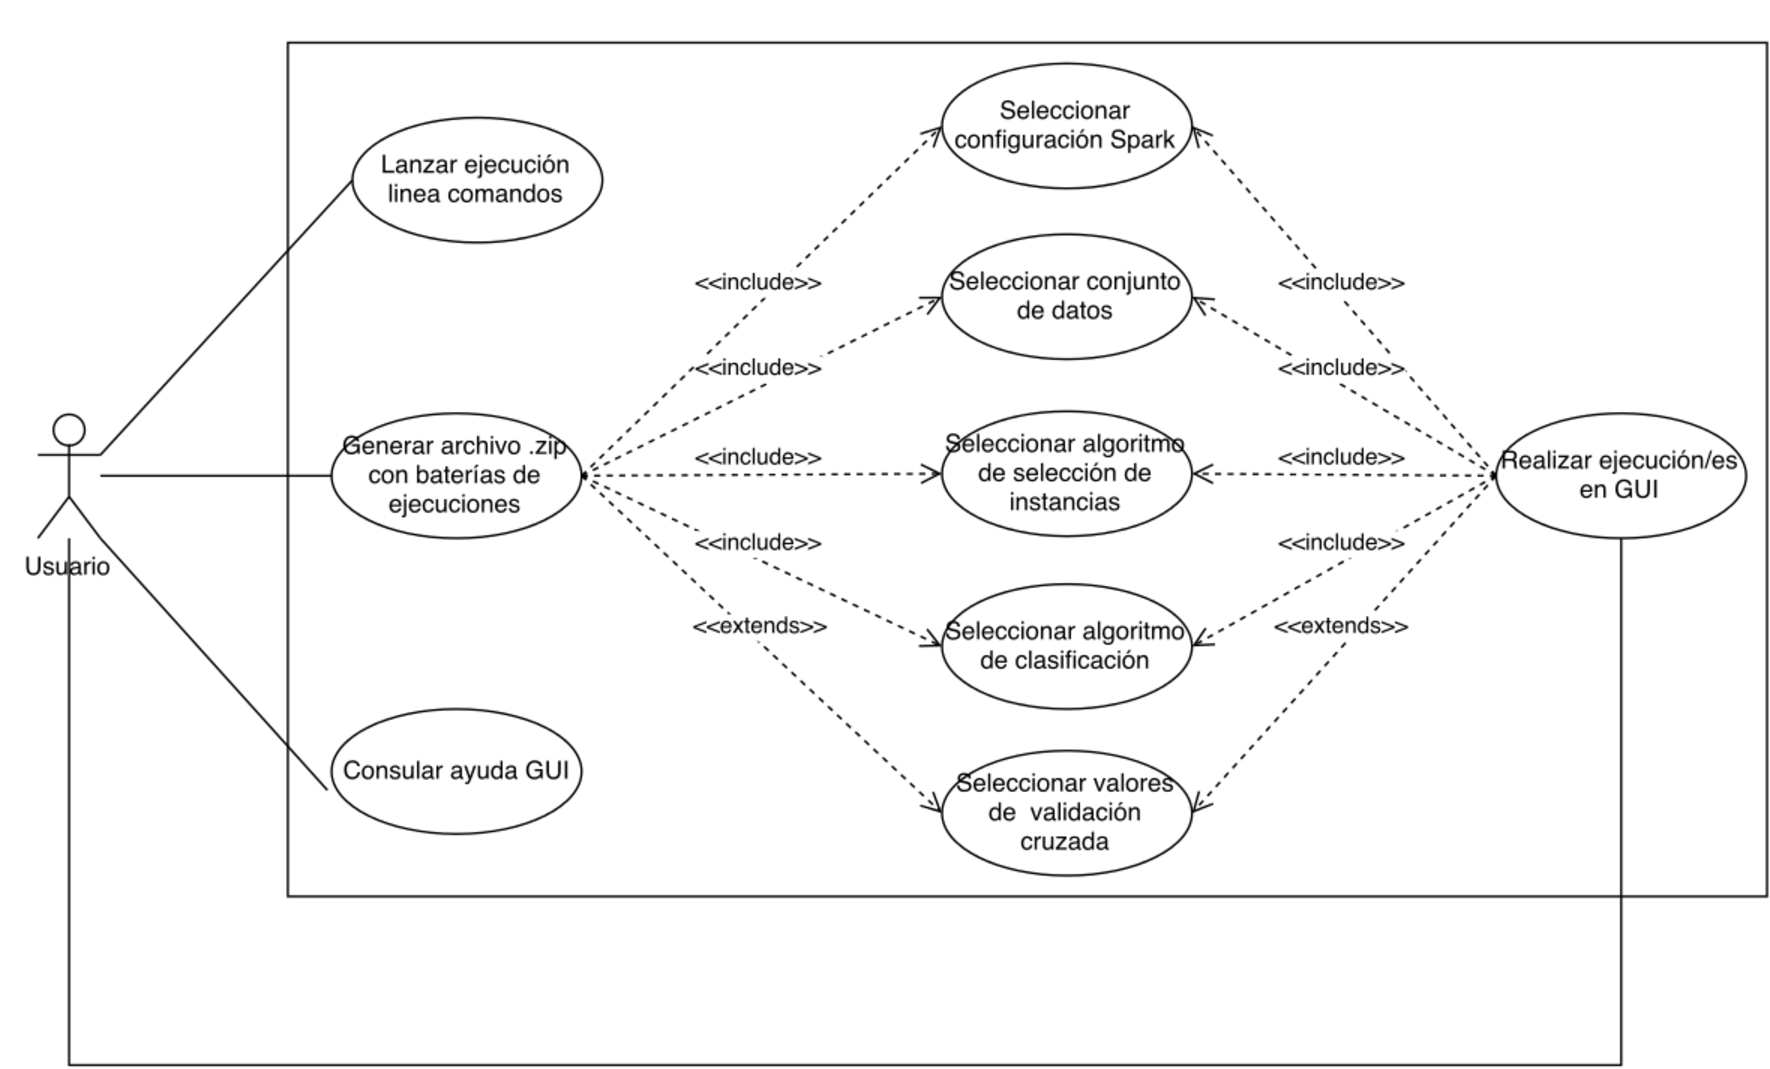
\includegraphics[width=1.0\textwidth]{img/anexo/diagrama_casos_de_uso}
		\caption{Diagrama de casos de uso.}\label{fig:img/anexo/diagrama_casos_de_uso}
	\end{figure}

%\imagen{img/anexo/diagrama_casos_de_uso}{Diagrama de casos de uso.}

 
\subsection{Casos de uso}
 
\begin{table}
  \begin{center}
   \begin{tabular}{|>{\cellcolor[gray]{0.8}} L{3cm} | L{9cm} |}
    \hline
    Caso de uso & Lanzar ejecución - Línea de comandos\\
    \hline
    Versión & 1.0 \\
    \hline
    Autor & Alejandro González Rogel \\
    \hline
    Requisitos & RF-1\newline
		RF-1.1\newline
		RF-1.2\newline
		RF-1.3\newline
		RF-1.4\newline
		RF-1.5\newline
		RF-1.6\\
    \hline
    Descripción & El usuario puede realizar la invocación, por línea de comandos, de un nueva tarea que implique un selector de instancias y un clasificador. Para ello necesitará aportar, además, una lista de parámetros que permitan la configuración de todos los componentes involucrados.\\
    \hline
    Precondiciones & Ninguna \\
    \hline
    Acciones & 1. El usuario realiza el lanzamiento de la aplicación mediante consola de comandos usando el script ``spark-submit'' proporcionado por Spark. \newline
    2. La aplicación realiza la ejecución. \newline
    \hspace{1em} 2.1 Se muestra periodicamente, en mensajes por consola, el punto de la ejecución en el que nos encontramos. \newline
    \hspace{1em} 2.2 La aplicación escribe los resultados de la ejecución en un fichero.\newline
    \hspace{1em} 2.3 La aplicación muestra un último mensaje indicando la correcta ejecución.\\
    \hline
    Postcondiciones & Ningua \\
    \hline
    Excepciones & Los parámetros introducidos en la invocación del programa son erróneos. Se paralizará la ejecución y se informará mediante un mensaje por consola de comandos si este fuese el caso. \\
    \hline
    Importancia & Alta \\
    \hline
   \end{tabular}
   \caption{Caso de uso ``Lanzar ejecución - Línea de comandos''}
   \label{tabla:casoUso1}
  \end{center}
 \end{table} 
 
 
\begin{table}
  \begin{center}
   \begin{tabular}{|>{\cellcolor[gray]{0.8}} L{3cm} | L{9cm} |}
    \hline
    Caso de uso & Realizar ejecución/es GUI\\
    \hline
    Versión & 1.0 \\
    \hline
    Autor & Alejandro González Rogel \\
    \hline
    Requisitos & 
    		RF-2\newline
    		RF-2.1\newline
		RF-2.2\newline
		RF-2.3\newline
		RF-2.4\newline
		RF-2.5\newline
		RF-2.6\\
    \hline
    Descripción & Mediante el uso de la interfaz gráfica, el usuario puede programar una o varias ejecuciones y lanzarlas en el momento.\\
    \hline
    Precondiciones & El usuario ha iniciado la interfaz gráfica. \\
    \hline
    Acciones & 1. El usuario completa los campos de opciones comunes de Spark. \newline
    			   2. El usuario indica una o varias configuraciones de Spark \newline
    			   3. El usuario indica uno o varios conjuntos de datos \newline
    			   4. El usuario selecciona uno o varios selectores de instancias. \newline
    			   5. El usuario selecciona un clasificador. \newline
    			   6. El usuario puede indicar opciones para la validación cruzada (opcional). \newline
    			   7. El usuario presiona un botón para ejecutar las tareas programadas. \newline
    			   8. La aplicación informa cuando se finalice la operación.
    			   \\
    \hline
    Postcondiciones & Los resultados de la ejecución han sido almacenados en un fichero de texto en la ruta correspondiente. \\
    \hline
    Excepciones & Ninguna \\
    \hline
    Importancia & Baja \\
    \hline
   \end{tabular}
   \caption{Caso de uso ``Realizar ejecución/es GUI''}
   \label{tabla:casoUso2}
  \end{center}
 \end{table} 
 
 
\begin{table}
  \begin{center}
   \begin{tabular}{|>{\cellcolor[gray]{0.8}} L{3cm} | L{9cm} |}
    \hline
    Caso de uso & Generar archivo .zip con baterías de ejecuciones\\
    \hline
    Versión & 1.0 \\
    \hline
    Autor & Alejandro González Rogel \\
    \hline
    Requisitos & 
    		RF-2\newline
    		RF-2.1\newline
		RF-2.2\newline
		RF-2.3\newline
		RF-2.4\newline
		RF-2.5\newline
		RF-2.6\\
    \hline
    Descripción & Mediante el uso de la interfaz gráfica, el usuario puede programar una o varias ejecuciones y generar un archivo de extensión .zip que contendrá un script de lanzamiento y todos los conjuntos de datos necesarios para la ejecución.\\
    \hline
    Precondiciones & El usuario ha iniciado la interfaz gráfica. \\
    \hline
    Acciones & 1. El usuario completa los campos de opciones generales de Spark. \newline
    			   2. El usuario indica una o varias configuraciones de Spark \newline
    			   3. El usuario indica uno o varios conjuntos de datos \newline
    			   4. El usuario selecciona uno o varios selectores de instancias. \newline
    			   5. El usuario selecciona un clasificador. \newline
    			   6. El usuario puede indicar opciones para la validación cruzada (opcional). \newline
    			   7. El usuario presiona un botón para generar el archivo zip. \newline
    			   8. La aplicación informa cuando se finalice la operación.
    			   \\
    \hline
    Postcondiciones & Se ha generado un archivo de extensión .zip \\
    \hline
    Excepciones & Ninguna \\
    \hline
    Importancia & Media \\
    \hline
   \end{tabular}
   \caption{Caso de uso ``Generar archivo .zip con baterías de ejecuciones''}
   \label{tabla:casoUso3}
  \end{center}
 \end{table}  
 
 
 \begin{table}
  \begin{center}
   \begin{tabular}{|>{\cellcolor[gray]{0.8}} L{3cm} | L{9cm} |}
    \hline
    Caso de uso & Seleccionar configuración Spark\\
    \hline
    Versión & 1.0 \\
    \hline
    Autor & Alejandro González Rogel \\
    \hline
    Requisitos & RF-2\newline
    				 RF-2.1\newline
    				 RF-3\newline
    				 RF-3.1 \\
    \hline
    Descripción & El usuario puede indicar una configuración de Spark rellenando un conjunto de campos de texto. \\
    \hline
    Precondiciones & El usuario ha iniciado la interfaz gráfica.\\
    \hline
    Acciones & 1. El usuario ha presionado un botón para añadir una nueva configuración de Spark. \newline
    			   2. La aplicación muestra un nuevo diálogo. \newline
    			   3. El usuario rellena todos los campos mostrados en el nuevo diálogo. \newline
    			   4. El usuario presiona un botón para aceptar la nueva configuración.  \\
    \hline
    Postcondiciones & Una nueva configuración ha de haberse añadido a la lista de configuraciones. \\
    \hline
    Excepciones & Ninguna \\
    \hline
    Importancia & Baja \\
    \hline
   \end{tabular}
   \caption{Caso de uso ``Seleccionar configuración Spark''}
   \label{tabla:casoUso5}
  \end{center}
 \end{table}
 
  \begin{table}
  \begin{center}
   \begin{tabular}{|>{\cellcolor[gray]{0.8}} L{3cm} | L{9cm} |}
    \hline
    Caso de uso & Seleccionar conjunto de datos\\
    \hline
    Versión & 1.0 \\
    \hline
    Autor & Alejandro González Rogel \\
    \hline
    Requisitos & RF-2\newline
    				 RF-2.2\newline
    				 RF-3\newline
    				 RF-3.2 \\
    \hline
    Descripción & El usuario puede indicar un fichero que contenga un conjunto de datos así como algunos parámetros que permitan su lectura. \\
    \hline
    Precondiciones & El usuario ha iniciado la interfaz gráfica.\\
    \hline
    Acciones & 1. El usuario ha presionado un botón para añadir un nuevo conjunto de datos. \newline 
    2. La aplicación muestra un nuevo diálogo. \newline
    			   3. El usuario selecciona el botón para buscar en los archivos del sistema un conjunto de datos. Alternativamente, puede escribirlo manualmente. \newline
    			   4. El usuario cumplimenta todos los campos restantes mostrados en el diálogo. \newline
    			   5. El usuario presiona un botón para aceptar la nueva configuración. \\
    \hline
    Postcondiciones & Un nuevo conjunto de datos, junto con sus opciones de lectura, ha de haberse añadido a la lista de conjuntos de datos. \\
    \hline
    Excepciones & Ninguna \\
    \hline
    Importancia & Baja \\
    \hline
   \end{tabular}
   \caption{Caso de uso ``Seleccionar conjunto de datos''}
   \label{tabla:casoUso6}
  \end{center}
 \end{table}
 
 
   \begin{table}
  \begin{center}
   \begin{tabular}{|>{\cellcolor[gray]{0.8}} L{3cm} | L{9cm} |}
    \hline
    Caso de uso & Seleccionar algoritmo de selección de instancias\\
    \hline
    Versión & 1.0 \\
    \hline
    Autor & Alejandro González Rogel \\
    \hline
    Requisitos & RF-2\newline
    				 RF-2.3\newline
    				 RF-3\newline
    				 RF-3.3 \\
    \hline
    Descripción & El usuario puede seleccionar un algoritmo de selección de instancias de entre las posibles opciones y configurarlo para su ejecución. \\
    \hline
    Precondiciones & El usuario ha iniciado la interfaz gráfica.\\
    \hline
    		Acciones & 1.El usuario ha presionado el botón para añadir un nuevo selector de instancias.  \newline
    		
    		2. La aplicación muestra un nuevo diálogo. \newline
    		3. El usuario selecciona, tras pulsar el botón de selección, el filtro que desea. \newline
    		4. La aplicación añade nuevos campos al diálogo.
    		5. El usuario cumplimenta los nuevos campos mostrados en el diálogo. \newline
    		6. El usuario presiona un botón para aceptar la nueva configuración. \\
    \hline
    Postcondiciones & Un nuevo selector de instancias, junto con su configuración, ha de haberse añadido a la lista de conjuntos de datos. \\
    \hline
    Excepciones & Ninguna \\
    \hline
    Importancia & Baja \\
    \hline
   \end{tabular}
   \caption{Caso de uso ``Seleccionar algoritmo de selección de instancias''}
   \label{tabla:casoUso7}
  \end{center}
 \end{table}
 
    \begin{table}
  \begin{center}
   \begin{tabular}{|>{\cellcolor[gray]{0.8}} L{3cm} | L{9cm} |}
    \hline
    Caso de uso & Seleccionar algoritmo de clasificación.\\
    \hline
    Versión & 1.0 \\
    \hline
    Autor & Alejandro González Rogel \\
    \hline
    Requisitos & RF-2\newline
    				 RF-2.4\newline
    				 RF-3\newline
    				 RF-3.4 \\
    \hline
    Descripción & El usuario puede seleccionar un algoritmo de clasificación y configurarlo para su ejecución. \\
    \hline
    Precondiciones & El usuario ha iniciado la interfaz gráfica.\\
    \hline
    		Acciones & 1. El usuario presiona el botón que permite seleccionar entre los diferentes clasificadores posibles. \newline
    		2. El usuario selecciona un clasificador.\newline
    		3. La aplicación genera nuevos campos con las opciones de configuración del clasificador.\newline
    		4. El usuario rellena los campos con las opciones de configuración.    \\ 			
    \hline
    Postcondiciones & Ninguna\\
    \hline
    Excepciones & Ninguna \\
    \hline
    Importancia & Baja \\
    \hline
   \end{tabular}
   \caption{Caso de uso ``Seleccionar algoritmo de clasificación''}
   \label{tabla:casoUso8}
  \end{center}
 \end{table}
 
 
     \begin{table}
  \begin{center}
   \begin{tabular}{|>{\cellcolor[gray]{0.8}} L{3cm} | L{9cm} |}
    \hline
    Caso de uso & Seleccionar valores de validación cruzada.\\
    \hline
    Versión & 1.0 \\
    \hline
    Autor & Alejandro González Rogel \\
    \hline
    Requisitos & RF-2\newline
    				 RF-2.5\newline
    				 RF-3\newline
    				 RF-3.5 \\
    \hline
    Descripción & El usuario puede indicar una configuración de validación cruzada con la que realizar las ejecuciones. \\
    \hline
    Precondiciones & El usuario ha iniciado la interfaz gráfica.\\
    \hline
    		Acciones & 1. El usuario marca la opción que habilita la validación cruzada. \newline
    		2. El usuario cumplimenta los campos de configuración de la validación cruzada.\\
    \hline
    Postcondiciones & Ninguna\\
    \hline
    Excepciones & Ninguna \\
    \hline
    Importancia & Baja \\
    \hline
   \end{tabular}
   \caption{Caso de uso ``Seleccionar valores de validación cruzada''}
   \label{tabla:casoUso9}
  \end{center}
 \end{table}
 
 
 
 \begin{table}
  \begin{center}
   \begin{tabular}{|>{\cellcolor[gray]{0.8}} L{3cm} | L{9cm} |}
    \hline
    Caso de uso & Consultar ayuda GUI\\
    \hline
    Versión & 1.0 \\
    \hline
    Autor & Alejandro González Rogel \\
    \hline
    Requisitos & RF-4 \\
    \hline
    Descripción & El usuario puede consultar el funcionamiento de la interfaz gráfica mediante un botón de ayuda proporcionado en dicha interfaz.\\
    \hline
    Precondiciones & Se ha iniciado la interfaz gráfica. \\
    \hline
    Acciones & 1. El usuario presiona sobre el botón de ayuda en la interfaz. \newline
    				2. La aplicación muestra una nueva ventana con la ayuda.\\
    \hline
    Postcondiciones & Ninguna \\
    \hline
    Excepciones & Ninguna \\
    \hline
    Importancia & Baja \\
    \hline
   \end{tabular}
   \caption{Caso de uso ``Consultar ayuda GUI''}
   \label{tabla:casoUso4}
  \end{center}
 \end{table}
\apendice{Especificación de diseño}

\section{Introducción}

\section{Diseño de datos}

\section{Diseño procedimental}

\section{Diseño arquitectónico}



\apendice{Documentación técnica de programación}


\section{Introducción}

En este apéndice se van a describir todos aquellos aspectos que se consideren de interés para una persona que desee continuar el desarrollo del proyecto o quiera obtener un conocimiento más avanzado del mismo.

\section{Estructura de directorios}

A continuación se va a hacer mención a la funcionalidad de cada una de las carpetas que conforman el árbol de directorios de nuestro proyecto:

\begin{itemize}
	\item \textbf{src:} Carpeta destinada a almacenar el código fuente la aplicación.
	\begin{itemize}
		\item \textbf{main/scala:} Este directorio contendrá todos los ficheros fuente que estén escritos en Scala. Al no haberse usado ningún otro lenguaje ni contar con clases para realizar pruebas, este es el único directorio de la carpeta ``src''.
	\end{itemize}
	\item \textbf{resources:} Carpeta destinada a almacenar todos aquellos elementos que, sin ser código, también son necesarios para la ejecución del programa. Aquí podríamos incluir fichero .xml, html, imágenes o cualquier otro fichero multimedia, etc.
	\begin{itemize}
		\item \textbf{gui:} Contiene todos los recursos utilizados por la interfaz gráfica.
		\item \textbf{loggerStrings:} Almacena ficheros de texto con sentencias que pueden ser utilizadas por los diferentes \textit{logger} en diferentes clases de nuestro programa.
	\end{itemize}
	\item \textbf{target:} Contiene los archivos resultantes de aplicar alguna operación de Apache Maven sobre el proyecto (compilación, empaquetado o generación de documentación). Para más información al respecto visitar la sección \ref{subsec:compilacion}, situada en este mismo anexo.
	\begin{itemize}
		\item \textbf{site/scaladocs:} Ruta que contiene la documentación, generada por Scaladoc, de las clases del proyecto.
	\end{itemize}
\end{itemize}


\section{Manual del programador}

A lo largo de esta sección vamos a describir diferentes tareas que, si bien no se refieren directamente a la ejecución del programa, pueden conducir a un manejo más avanzado del mismo.

Antes de proceder es necesario comprender y haber realizado el proceso de instalación de todos los componentes mencionados en la sección \ref{sec:Instalacion}, independientemente de si esos componentes han sido marcados como opcionales o no para el usuario normal.

\subsection{Configurando Spark para guardar información sobre ejecuciones}\label{subsec:configurandoSpark}

Con la configuración por defecto, Spark apenas almacena información sobre las ejecuciones realizadas, pudiendo acceder a parámetros sobre la ejecución solo mientras el programa está corriendo. A lo largo de esta sección explicaremos que es posible modificar este comportamiento y la manera de lograrlo.

Lo primero que necesitamos es modificar algunas propiedades de Spark. En su carpeta de configuración  (\textit{\$SPARK\_HOME/conf}) debemos buscar un fichero por nombre ``spark-defaults.conf''. Si es la primera vez que realizamos este tipo de operaciones es posible que este fichero no exista, haciendo necesario crearlo nosotros mismos o renombrar el fichero ``spark-defaults.conf.template'' que actúa de ejemplo y está situado en la misma carpeta.

Sea cual sea la opción elegida, en nuestro fichero de configuración ``spark-defaults.conf'' escribiremos las siguientes líneas:

\begin{lstlisting}[basicstyle=\small]
spark.eventLog.enabled	true
spark.eventLog.dir	    /opt/spark-1.5.1/logs/exec-logs
spark.history.fs.logDirectory /opt/spark-1.5.1/logs/exec-logs
\end{lstlisting}

La primera línea es obligatoria y no admite cambios. Las dos siguientes sirven para indicar el fichero donde deseamos almacenar la información de las ejecuciones. La ruta seleccionada es indiferente, pero es necesario destacar dos aspectos:
\begin{itemize}
\item Las dos rutas indicadas han de ser iguales.
\item Las rutas han de apuntar a un directorio existente. Si indicamos una ruta inexistente Spark no generará los directorios que falten, sino que emitirá un error cuando intentemos ejecutar una aplicación y esta quiera guardar sus datos de ejecución. Es por ello que, en el caso concreto de la configuración ofrecida como ejemplo, deberíamos crear la carpeta ``exec-logs'' en  \textit{/opt/spark-1.5.1/logs} antes de proceder.
\end{itemize}

Con esto, deberíamos contar con toda la información de nuestras ejecuciones aun después de que estas hayan acabado. Será en la siguiente sección cuando hablaremos de cómo acceder a todos estos datos para su posterior análisis.


\subsection{Monitorización y análisis}\label{subsec:monitorizacion}

Un aspecto clave en el desarrollo de aplicaciones para \textit{big data} es el de controlar y analizar el rendimiento de los algoritmos. Para ello, vamos a explicar en la siguiente sección como acceder a este tipo de información. No es objetivo de este anexo, sin embargo, explicar toda la información analizable ni la manera en la que ésta se organiza.

Antes de continuar, es necesario indicar que toda esta información proporcionada aquí corresponde a la manera de analizar una aplicación ejecutada en el modo \textit{Standalone} de Spark (ver sección \ref{subsec:modosDespliegueSpark} para más información). Si Spark se ejecutase usando algún administrador de clústeres el modo de acceder a la información podría ser distinto dependiendo del software usado. Igualmente, si ejecutamos en modo local no existe una manera de acceder a los datos de análisis una vez la aplicación ha finalizado su ejecución.

Con todo, comenzaremos contemplando la posibilidad de observar la ejecución de un programa mientras éste está todavía en ejecución. Esto puede hacerse accediendo, mediante el navegador, a la ruta \url{http://localhost:4040} (suponemos que nuestra máquina es el nodo maestro). Podemos ver un ejemplo de la página inicial en la imagen \ref{fig:img/anexo/pantalla_4040}. Esta información solo estará disponible mientras la aplicación lanzada siga ejecutando, y toda la información que podemos ver será borrada si no hemos seguido los pasos descritos en la anterior subsección.

\imagen{img/anexo/pantalla_4040}{Ejemplo de monitorización de una aplicación en marcha.}

Suponiendo que queremos realizar un análisis de todas las aplicaciones que han sido lanzadas en la red de nodos en modo \textit{Standalone}, podemos hacerlo consultado la dirección \url{http://localhost:8080}. Además de información referente a nuestro clúster, podemos observar un listado de aplicaciones ejecutadas o en ejecución, a cuya información se puede acceder pulsando sobre cualquiera de ellas (ver imagen \ref{fig:img/anexo/pantalla_8080}).

\imagen{img/anexo/pantalla_8080}{Pantalla de inicio de un clúster Standalone.}

De nuevo, la ruta indicada ruta es válida si únicamente estamos trabajando en la máquina local o somos el nodo maestro de la red. Igualmente, volvemos a recordar que hemos tenido que habilitar la opción de Spark para guardar información de las ejecuciones.

Por último, si deseamos acceder a toda la información de ejecuciones guardada en nuestra máquina, independiente de si continuamos formando parte de una red de nodos o hemos sido el nodo maestro de varias redes, podemos accederlo iniciando el servicio ``History Server'' y accediendo a la ruta (\url{http://localhost:18080/}), donde se nos mostrará un listado con todas las aplicaciones ejecutadas de las que se tiene información. Para iniciar el servicio mencionado, desde consola de comandos, debemos escribir el comando:

\begin{lstlisting}[language=bash]
$ $SPARK_HOME/sbin/start-history-server.sh
\end{lstlisting}

Podemos ver un ejemplo del histórico de ejecuciones en la imagen \ref{fig:img/anexo/pantalla_18080}.

\imagen{img/anexo/pantalla_18080}{Ejemplo de la interfaz del servidor de históricos.}

\section{Compilación, instalación y ejecución}

A lo largo de esta sección vamos a hablar de todos los pasos necesarios para poder trabajar sobre el código del proyecto. Esto incluye la instalación de diferentes componentes, la configuración del entorno de desarrollo y la comprensión de la herramienta Apache Maven como administrador en labores como la compilación.

\subsection{Instalación}

Si deseamos trabajar sobre el código del proyecto, además de necesitar todos los materiales definidos en la sección \ref{sec:Instalacion} vamos a necesitar los definidos en este apartado.

\subsubsection{Scala 2.11.7}
Aunque podemos descargar la última versión de Scala desde la página oficial (\url{http://www.scala-lang.org/}), la descarga que se nos ofrece por defecto es un archivo .tar.gz que nos obligaría a realizar toda la instalación manualmente (suponiendo que estamos en un sistema Ubuntu como el utilizado durante el proyecto).

Por ello, vamos a realizar la instalación mediante un archivo .deb (paquete Debian) que también puede ser utilizado por nuestro sistema y que nos ahorrará realizar la instalación manualmente. Podemos acceder al repositorio que guarda este paquete desde un navegador (\url{http://www.scala-lang.org/files/archive/}) o descargarlo mediante el siguiente comando:

\begin{lstlisting}[language=bash]
$ wget www.scala-lang.org/files/archive/scala-2.11.7.deb
\end{lstlisting}

Independientemente del método seguido, una vez tengamos el archivo en nuestro ordenador ejecutamos el siguiente comando desde la carpeta que contenga el paquete .deb:

\begin{lstlisting}[language=bash]
$ sudo dpkg -i scala-2.11.7.deb
\end{lstlisting}

Si todo ha salido correctamente, una vez termine de ejecutarse la orden anterior podemos ejecutar el comando \textit{scala -version} y esperar una salida similar a esta:

\begin{lstlisting}[language=bash]
$ scala -version
Scala code runner version 2.11.7 -- Copyright 2002-2013
\end{lstlisting}

Recordar que, en el caso de utilizar cualquier otra versión de Scala, esta tiene que ser compatible con la versión Java que se encuentre instalada. Por ejemplo, Java 8 solo puede ser utilizado a partir de versiones 2.11 y será obligatorio a partir de la versión de Scala 2.12. \cite{Scala2.12Roadmap}

\subsubsection{Scala IDE}

Scala IDE es el entorno de desarrollo utilizado durante el proyecto.

Descargaremos la  última versión disponible del producto desde su página oficial: \url{http://scala-ide.org/}

Dentro de las posibles descargas que podemos seleccionar, elegiremos aquella que esté destinada a nuestro sistema operativo, en nuestro caso concreto, ``Linux - 64 bits''. Al descargar esta herramienta, en realidad estamos descargando el entorno de desarrollo Eclipse (\url{https://eclipse.org/}) con una serie de \textit{plugins} añadidos, entre los que destaca el llamado Scala IDE.

Una vez descargado, descomprimiremos el archivo en la ruta \textit{/opt}. Mediante línea de comandos podemos hacerlo utilizando la siguiente sentencia:

\begin{lstlisting}
$ cd /opt/ && sudo tar -zxvf \
~/Downloads/scala-SDK-4.2.0-vfinal-2.11-\
linux.gtk.x86_64.tar.gz
\end{lstlisting}

Recuerde que el código puede cambiar dependiendo del nombre del archivo que sea descargado o del directorio donde se encuentre.

\subsection{Importando el proyecto en Scala IDE}


Suponiendo que se ha seguido la instalación del entorno de desarrollo mencionado (Scala IDE) seguiremos los siguientes pasos para importar y ejecutar nuestro proyecto desde el propio programa.

Primero de todo, para importar el código a nuestro lugar de trabajo debemos dirigirnos al menú superior, opción ``File'' y, de entre las alternativas del menú desplegable, seleccionar ``Import''. Alternativamente también podemos abrir el menú desplegable haciendo clic derecho sobre el panel de nombre ``Package explorer'', situado generalmente a la izquierda de la pantalla.

Veremos un nuevo diálogo similar al mostrado en la figura \ref{fig:img/anexo/existing_maven_projects}, donde seleccionaremos, entre todas las opciones, aquella que diga ``Existing Maven Projects''. Posteriormente, presionamos sobre el botón ``Next'' para continuar.

\imagen{img/anexo/existing_maven_projects}{Diálogo para seleccionar un médoto de importación en Eclipse IDE.}

En el nuevo diálogo presionaremos sobre el botón ``Browse'' para indicar el directorio principal de nuestro proyecto. Si todo es correcto, una vez seleccionemos la carpeta que deseemos el resultado debería ser similar al mostrado en la imagen \ref{fig:img/anexo/proyecto_importado}.

\imagen{img/anexo/proyecto_importado}{Diálogo para importar un proyecto al entorno Eclipse IDE.}

Pulsamos sobre el botón de finalizar y, si todo ha salido correctamente, deberíamos poder ver nuestro proyecto en el menú lateral izquierdo, tal como muestra \ref{fig:img/anexo/paquete_importado}

\imagen{img/anexo/paquete_importado}{Paquete importado en el menú lateral.}


\subsection{Ejecutando el proyecto en Scala IDE}

Como puede observarse en el manual del usuario (\ref{sec:manualUsuario}) el lanzamiento de una aplicación en Spark se realiza mediante un script que proporciona el propio Spark y en el cual se pueden indicar ciertos parámetros de ejecución. Por ello, para el lanzamiento del programa desde Eclipse hemos de modificar añadir algún fragmento de código que genere una configuración de Spark que, en cualquier otro método de lanzamiento, es creada por el script utilizado.

Para ello hemos de modificar un fragmento de código en la clase \textit{ISClassExec} del paquete \textit{launcher.execution}, tal y como puede verse en \ref{lst:codigoSpark} y \ref{lst:codigoSpark2}


\begin{lstlisting}[language=Java,tabsize=4,frame = single,caption=Código para la ejecución del programa mediante el script ``spark-sumbit''. ,captionpos=b,label=lst:codigoSpark]
val sc = new SparkContext()
\end{lstlisting}

\begin{lstlisting}[language=Java,tabsize=4,frame = single,caption=Ejemplo de código para la ejecución del programa desde Eclipse. ,captionpos=b,label=lst:codigoSpark2]
	val master = "local[2]"
    val sparkConf =
  	  new SparkConf().setMaster(master)
  	  .setAppName("Prueba_Eclipse")
    val sc = new SparkContext(sparkConf)
\end{lstlisting}

Ahora, debemos indicar, de manera manual, cuál será la clase principal que deseamos lanzar. Es posible que esto cambie de acuerdo al tipo de ejecución que queremos realizar (lanzar la interfaz gráfica o un experimento de Spark), pero los pasos a seguir son idénticos.

Desde la pantalla de Scala IDE nos dirigiremos al menú superior, presionamos sobre ``Run'' y seleccionamos la opción ``Run configurations''. Esto abrirá una nueva ventana similar a la mostrada en la figura \ref{fig:img/anexo/run_configurations}.

Presionando dos veces sobre el texto ``Scala application'', en el menú izquierdo, podremos generar una nueva configuración para el proyecto. Allí rellenaremos los campos requeridos, con especial interés al campo ``Main Class'', que deberá escribirse manualmente porque el entorno no detecta ninguna de las clases principales de los proyectos. En nuestro caso, ese campo siempre será \textit{launcher.ExperimentLauncher} para lanzar experimentos y \textit{gui.SparkISGUI} para lanzar la interfaz gráfica.


\imagen{img/anexo/run_configurations}{Ventana de configuración de ejecuciones en Scala IDE.}


Finalmente, si deseamos introducir argumentos al iniciar una ejecución, podemos hacerlo desde la pestaña ``Arguments'', en la ventana anterior, rellenando el campo ``Program arguments'' con la información que deseemos (ver ejemplo en \ref{fig:img/anexo/arguments_configuration})

\imagen{img/anexo/arguments_configuration}{Ventana de configuración de ejecuciones en Scala IDE - Argumentos.}


Con todo definido, podemos presionar sobre el botón ``Run'' para comenzar a ejecutar nuestro programa.

Para posteriores ejecuciones no necesitaremos volver a definir de nuevo todo el proceso, sino que la opción será guardada y podrá ser accedida de manera sencilla seleccionándola desde el menú desplegable que proporciona el botón de ejecutar en el menú superior de Eclipse (ver figura \ref{fig:img/anexo/menu_superior_eclipse}).

	\begin{figure}[!h]
		\centering
		
\includegraphics[width=0.4\textwidth]{img/anexo/menu_superior_eclipse}
		\caption{Fragmento del menú superior de Scala IDE.}\label{fig:img/anexo/menu_superior_eclipse}
	\end{figure}
	
Si tenemos configurado el entorno para no realizar la compilación automática de las clases o hemos modificado algún recurso, debe realizarse una acción anterior al lanzamiento de cualquier ejecución. Desde la ventana principal del entorno de desarrollo, haremos clic con el botón derecho sobre la carpeta de nuestro proyecto, ``Run as'', ``Maven build''. Se nos abrirá una ventana similar a la mostrada en la figura \ref{fig:img/anexo/eclipse_maven}.
	
	\imagen{img/anexo/eclipse_maven}{Ventana de configuración de Maven.}
	
Simplemente, necesitamos escribir en el campo de texto ``Goals'' los objetivos ``clean package'' y presionar sobre el botón ``Run''. Esto debería realizar la compilación de todo el proyecto desde el entorno de desarrollo.

	
	\subsection{Compilación}\label{subsec:compilacion}

Para realizar la labor de compilación vamos a necesitar del software Apache Maven, cuya instalación ha sido indicada en \ref{subsec:instalaMaven}. Una vez contemos con este requisito la operación será prácticamente automática.

Desde consola nos dirigimos al directorio raíz donde esté situado el proyecto. Una vez allí, ejecutamos el comando siguiente:

\begin{lstlisting}[language=bash]
$ mvn clean package
\end{lstlisting}

Si es la primera vez que se realiza esta operación sobre el proyecto, o incluso la primera vez que se utiliza Maven, es muy probable que se requiera de algo de tiempo adicional mientras se descargan todos los materiales necesarios para poder llevar a cabo la labor de compilación.

Toda la información referente a la administración del proyecto (dependencias, fases, etc.) debe encontrarse en el documento situado en la carpeta raíz. El nombre de este documento suele ser ``pom.xml'' pero, dado que en este proyecto existen diferentes distribuciones finales y un fichero de este tipo solo debería generar una única distribución, si deseamos utilizar cualquier otro fichero de los proporcionados para administrar el proceso deberemos ejecutar el comando:

\begin{lstlisting}[language=bash]
$ mvn -f otro_pom.cml clean package
\end{lstlisting}

Actualmente se cuentan con los siguientes ficheros para generar distribuciones:
\begin{itemize}
\item \textbf{pom.xml:} Realiza una compilación y empaquetado de todo el material del proyecto. Debe encontrarse instalada la versión de Scala 2.11 para realizar la compilación.
\item \textbf{pom\_gui.xml:} Genera una distribución que contará únicamente con los componentes gráficos del sistema. Vuelve a ser requerido Scala 2.11 para la fase de compilación.
\item \textbf{pom\_cluster.xml:} Crea una distribución que contendrá todos los elementos menos los relacionados con la interfaz gráfica. La compilación ha de realizarse esta vez con Scala 2.10, por ser la versión que necesitan los servicios que hemos utilizado.
\end{itemize}

\subsection{Generando documentación}\label{subsec:documentacion}

De nuevo mediante el uso de Apache Maven, podemos obtener la documentación de las clases del proyecto utilizando el siguiente comando desde el directorio raíz del proyecto:

\begin{lstlisting}[language=bash]
$ mvn clean scala:doc@Scaladoc
\end{lstlisting}

La documentación será generada en la carpeta \textit{target/sites/scaladocs} utilizando el software ``Scaladoc''.

Es necesario indicar que este generador de documentación tiene algunos inconvenientes:
\begin{itemize}
\item El programa ignora cualquier variable, método o clase privada, sin la posibilidad de poder revertir esta opción. Es por ello que cualquier material marcado como privado no aparecerá en los documentos generados.
\item Por defecto, los dicheros generados mostrarán todos los métodos de una clase: los definidos y los heredados de cualquier otro componente, aunque no pertenezca a nuestra librería. Esto puede llegar a resultar molesto en algunas clases, como las pertenecientes a la interfaz gráfica. En este caso, podemos presionar sobre el botón ``Hide all'' que encontraremos en cada fichero html generado y que permite ocultar todos aquellos métodos o atributos heredados de componentes que, por lo general, no suelen interesarnos.
\end{itemize}
 

\imagen{img/anexo/scaladoc}{Página principal de la documentación con Scaladoc.}

\section{Otros aspectos relevantes a la hora de implementar}

Por parte del programador, es necesario conocer una serie de aspectos que han influido en la implementación actual del código y que podrían seguir siendo influyentes si se continuase el trabajo.

\subsection{Comprobar medidas estáticas de calidad}

A la hora de trabajar sobre el proyecto, se ha utilizado una herramienta llamada Scalastyle (\url{http://www.scalastyle.org/}) para buscar aspectos del código que afecten negativamente al programa y, sobretodo, a las futuras labores de mantenimiento. Su funcionamiento se basa en comprobar una serie de reglas a lo largo de los ficheros fuente del proyecto. Dichas reglas estarán definidas en un fichero de nombre ``scalastyle\_config.xml'' en el directorio raíz del proyecto.

El material proporcionado en el repositorio ofrece un archivo con las reglas utilizadas en este proyecto y se ha dejado la puerta abierta a poder chequear el código mediante la siguiente secuencia en consola:

\begin{lstlisting}[language=bash]
$ mvn verify
\end{lstlisting}

Esta operación generará una salida bajo el nombre de ``scalastyle-output.xml'' que contendrá un informe con todos los casos en los que las reglas definidas no se estén cumpliendo.

\subsection{Versión de Scala}

Uno de los problemas a los que se enfrenta este proyecto se encuentra con la versión de Scala utilizada para compilar las clases. Scala 2.10 y Scala 2.11 no producen binarios compatibles, lo que impide que programas escritos en la versión anterior puedan ser leídos cuando esperamos clases compiladas para Scala 2.11 y viceversa.

Se comenzó el proyecto utilizando la versión de Scala 2.11 y, por lo tanto, se configuró Spark para trabajar con esa misma versión. Sin embargo, nos hemos encontrado con la necesidad de ejecutar el proyecto en sistemas donde Spark continua utilizando Scala 2.10.

Este cambio de versiones, además de afectar a la manera en la que debemos compilar el proyecto, tiene influencia a la hora de programar, pues podemos encontrar clases que cumplan su función en una versión y resulten en algún error en la siguiente. 

Pensemos, por ejemplo, en la clase \textit{scala.util.Random}, cuya versión en Scala 2.10 no es serializable, mientras que en su versión siguiente sí lo es. Esto hace que, en caso de querer distribuir dicha clase entre un grupo de nodos, la acción resulte en error con versiones anteriores a Scala 2.11. En este caso concreto, se ha suprimido el uso de la clase \textit{scala.util.Random} para ser sustituido por \textit{java.util.Random}, que no presenta este tipo de problemas.

No se han encontrado más clases que ocasionen errores de compatibilidad pero se advierte este problema como medida de precaución para futuras iteraciones.

\subsection{Incluir nuevos algoritmos}

Un aspecto que puede resultar de interés para el programador es conocer como añadir nuevos algoritmos a la librería. Esto es sencillo y únicamente consta de dos requisitos:

\begin{itemize}
\item En primer lugar, sea cual sea el tipo de algoritmo que deseamos implementar, ha de heredar de la clase ``Trait''\footnote{Las clases ``Trait'' en Scala son similares a las clases ``Interfaze'' en Java} que le corresponda, implementando todos los métodos que se reciben de esa clase.
	\begin{itemize}
		\item Los algoritmos de selección de instancias paralelos deberán heredar de \textit{instanceSelection.abstr.TraitIS}.
		\item Los algoritmos de selección de instancias secuenciales deberán heredar de \textit{instanceSelection.seq.abstr.TraitSeqIS}.
		\item Al no existir ningún algoritmo de clasificación paralelo, no existe interfaz definida de la que heredar.
		\item Los algoritmos de clasificación secuenciales deben heredar de \textit{classification.seq.abstr.TraitSeqClassifier}.
		\item No existen otro tipo de elementos, como por ejemplo filtros de atributos, y por lo tanto tampoco no cuentan con una interfaz definida.
	\end{itemize} 
\item Para que los algoritmos sean reconocidos por la interfaz gráfica han de ser definidos en unos ficheros .xml situados en la carpeta ``resources'' bajo el nombre de ``availableFilters.xml'' o ``availableClassifiers.xml''. En estos ficheros habrá que indicar la ruta a nuestro algoritmo, así como alguna información sobre sus parámetros configurables. Podemos ver un ejemplo de la estructura de los ficheros .xml en el siguiente código:

\begin{lstlisting}[language=xml,keywordstyle=\color{black}]

<algorithms>
  ...
  <algorithm>
    <name>paquete.sub1.sub2.Clase</name>
	  <options>
		<option>
		  <name>Opción 1</name>
		  <description>Def</description>
		  <command>-com</command>
		  <default>1</default>
		  <optionType>1</optionType>
		</option>
	  </options>
	</algorithm>
	...
</algorithms>

\end{lstlisting}

La utilidad de cada etiqueta viene definida al inicio de los propios ficheros.

\end{itemize}


\subsection{\textit{k}-folds en la validación cruzada}

Uno de los problemas que ya hemos mencionado anteriormente tanto en otros anexos como en la propia memoria, es que Spark todavía se encuentra en un estado inicial donde algunos de los recursos que proporciona son escasos.

Quiero destacar el caso de la función \textit{kfolds} que podemos encontrarnos en la clase \textit{org.apache.spark.mllib.util.MLUtils} de la librería de Spark. Esta función, en la versión que hemos trabajado con Spark, se encuentra en estado ``experimental'' según la propia documentación de la clase \cite{SparkMLUtils}.

Se ha probado y demostrado durante este proyecto que la implementación actual de este método dista mucho de la implementación en Weka, la alternativa secuencial a Spark que hemos utilizado en este proyecto. Los \textit{k}-folds generados por Spark dividen el subconjunto inicial de tal manera que el resultado de clasificación final de nuestros experimentos se ve gravemente perjudicado. Se atribuye esto a que la función en Spark no realiza divisiones estratificadas, esto es, divisiones donde la proporción de un determinado tipo de instancias en el subconjunto final es similar a su proporción en el conjunto completo.

Como la finalidad de este proyecto no ha sido la de profundizar sobre este aspecto, se ha implementado una manera de crear los \textit{k}-folds utilizando otras operaciones de Spark (función ``sample'' de la estructuras RDD) y algunas operaciones sobre conjuntos. Si bien la solución aportada parece haber resuelto el problema, es necesario indicar que genera problemas en conjuntos de datos donde las instancias recogidas están repetidas muchas veces dentro del conjunto de datos.

Por todo esto, se anima al futuro programador a comprobar el funcionamiento de la función \textit{kfolds} que proporcione Spark o a tener en cuenta las limitaciones de la implementación proporcionada.

\subsection{Medición de tiempos de filtrado usando ISClassExecTest} \label{subsec:ISClassExecTest}

Puede ser de interés para el programador conocer la razón por la cual la clase \textit{launcher.execution.ISClassExecTest}, destinada a medir el tiempo de ejecución de la selección de instancias, posee una serie de operaciones que no se encuentran incluidas en la versión principal (\textit{launcher.execution.ISClassExec}).

Consideremos el siguiente fragmento de código, encargado de realizar la medición del tiempo que tardamos en filtrar un conjunto de datos de nombre ``train''

\begin{lstlisting}[float,language=Java,tabsize=4,frame = single,caption=Código de medición de tiempo de filtrado ,captionpos=b,label=lst:codigoEclipse]
    train.persist()
    train.name = "TrainData"
    train.foreachPartition { x => None }

    // Instanciamos y utilizamos el selector de instancias
    val start = System.currentTimeMillis
    val resultInstSelector = applyInstSelector(instSelector, train, sc).persist
    resultInstSelector.foreachPartition { x => None }
    executionTimes += System.currentTimeMillis - start
\end{lstlisting}

Pueden observarse varias cosas que no vemos en una ejecución normal:
\begin{itemize}
	\item El conjunto de datos ``train'' se persiste antes de iniciar la medición. Esto se realiza para estar seguros de que, a la hora de medir los tiempos de ejecución, nuestro conjunto de datos estará distribuido completamente entre nuestros nodos.
	\item Se realizan una serie de operaciones sin aparente sentido, pues vemos hasta en dos ocasiones la sentencia \textit{foreachPartition \{ x $=>$ None \}} que, teóricamente, manda hacer ``nada'' a cada partición. En realidad, esta sentencia tiene como finalidad forzar a Spark a realizar todas las operaciones necesarias para calcular la estructura RDD sobre la que se está aplicando antes de poder continuar. Puede parecer un tema trivial pero eliminar la sentencia puede influir en las mediciones realizadas, pues en ocasiones medirían operaciones que no deseamos tener en consideración y que deseamos que se ejecuten antes de comenzar a medir el tiempo.
\end{itemize}


Es necesario comprender que la clase \textit{ISClassExecTest} fue creada con la intención de medir de la manera más precisa posible los tiempos de ejecución del filtrado en Spark. Sin embargo, en tareas de \textit{big data}, esto no es lo habitual, pues una precisión medida en milisegundos no tiene sentido cuando las ejecuciones pueden durar días. Es por ello que, para mediciones que no requieran gran precisión, se aconseja utilizar la información que presentan las herramientas de monitorización de Spark (ver subsección \ref{subsec:monitorizacion}).

\apendice{Pruebas del sistema}\label{anexo:Pruebas}

\section{Introducción}

A lo largo de este proyecto, se han realizado una serie de mediciones cuyo objetivo principal consistió en comparar el comportamiento entre ejecuciones secuenciales y paralelas en tareas de minería. A lo largo de esta sección, vamos a mostrar todos los experimentos realizados, junto con una descripción de los elementos involucrados y las conclusiones extraídas.

Podemos diferenciar entre tres grandes comparaciones:

\begin{itemize}
	\item \textbf{Comparativa entre las herramientas utilizadas:} Utilizando material ya incluido en las bibliotecas de Weka y Spark, se ha realizado una comparación entre ambas tecnologías. Tendremos en cuenta, no solo el tiempo de ejecución, sino otros factores tales como el uso de memoria o el funcionamiento de los hilos de ejecución (con especial interés en su comportamiento con Spark)
	\item \textbf{Comparativa entre las ejecuciones, en una sola máquina, de los algoritmos LSHIS y DemoIS según sea su implementación secuencial o paralela:} En este caso, nuestro objetivo principal será comparar tiempos de ejecución del algoritmo de filtrado, aunque también tendremos en cuenta parámetros otros parámetros que puedan demostrar el buen funcionamiento de nuestra implementación.
	\item \textbf{Comparativa entre las ejecuciones en un clúster de los algoritmos LSHIS y DemoIS según su implementación secuencial o paralela:} Al igual que en el caso anterior, el objetivo principal en este caso es medir el tiempo de ejecución de la operación de selección de instancias.

\end{itemize} 

\section{Conjuntos de datos}\label{sec:ConjuntosDeDatos}

Los conjuntos de datos (\textit{datasets}), ordenados de menor a mayor según el número total de instancias de cada uno, pueden encontrarse en la tabla \ref{tabla:ConjuntosWekaSpark}. No todos los conjuntos han sido utilizados en todas las comparaciones, puesto que  algunas ejecuciones podrían no acabar en un tiempo prudencial. Por ello, en cada prueba vendrá especificado qué datasets han sido usados.

Indicar que, a la hora de seleccionar los conjuntos, se han elegido aquellos que compartan algunas características comunes:

\begin{itemize}
	\item No existen campos de tipo texto.
	\item No existen campos vacíos en ninguna de las instancias de los atributos.
\end{itemize}

Además, es importante indicar que todos los atributos han sido normalizados antes de realizar las mediciones.


\tablaSmall{Conjuntos de datos utilizados para la comparación entre Weka y Spark.}{L{5.55cm} R{2.35cm} m{2.35cm} m{2.35cm}}{ConjuntosWekaSpark}
{\centering Nombre del conjunto & \centering Instancias & \centering Atributos  & \multicolumn{1}{c}{Clases} \\}{

Iris & 150 & \centering 4 & \multicolumn{1}{c}{3}  \\ [0.2cm]
Image Segmentation \cite{Lichman:2013} & 2,310 & \centering 19 & \multicolumn{1}{c}{7}  \\ [0.2cm]
Banana shaped \cite{BananaDataset} & 5,300 & \centering 2 & \multicolumn{1}{c}{2}  \\ [0.2cm]
Pen-Based Recognition of Handwritten Digits \cite{Lichman:2013} & 10,992 & \centering 16 & \multicolumn{1}{c}{10}  \\ [0.2cm]
Letter Recognition \cite{Lichman:2013} & 20,000 & \centering 16 & \multicolumn{1}{c}{26}  \\ [0.2cm]
Human Activity Recognition \cite{HumanActivityDataset} & 165,632 & \centering 17 & \multicolumn{1}{c}{5}   \\ [0.2cm]
Covertype \cite{Lichman:2013} & 581,012 & \centering 54 & \multicolumn{1}{c}{6}  \\ [0.2cm]
Poker \cite{Lichman:2013} & 1,025,010 & \centering 10 & \multicolumn{1}{c}{10}  \\ [0.2cm]
HIGGS \cite{Lichman:2013} \cite{HIGGSDataSet} & 11,000,000\tablefootnote{El conjunto original consta de 11,000,000 instancias, pero por lo general se he reducido su tamaño original para acercarlo más al tamaño de los otros conjuntos. Cualquier cambio será especificado en la medición a la que afecte.} & \centering 28 & \multicolumn{1}{c}{2} \\ [0.2cm]

}

\section{Entorno de las pruebas}

Aunque cada medición tiene una serie características únicas que vendrán definidas en la subsección correspondiente, existen algunas circunstancias que son comunes a todas ellas:

\begin{itemize}
	\item El formato utilizado en los ficheros que contienen datos ha sido .arff para Weka y .csv para Spark. La razón por la que no se han utilizado ficheros .csv en Weka ha sido por la posibilidad de que esto produzca errores a la hora de leer el archivo~\cite{CSVWeka}.
	\item Para todas las pruebas hemos usado una validación cruzada 10x2.
	\item Como ya ha sido mencionado anteriormente, todos los atributos de los conjuntos de datos utilizados han sido normalizados previamente.
	\item En ejecuciones locales (ver experimento \ref{sec:wekaSparkComp} y \ref{sec:pruebasLSHISyDemoIS}) las pruebas se han realizado en un ordenador con capacidad para soportar hasta cuatro hilos simultáneamente y una memoria RAM de 8GB.
	\item En todas las ejecuciones hemos contado con memoria suficiente como para poder incluir en ella todo el conjunto de datos. Es necesario destacar que, pese a todo, este supuesto no es común dentro del \textit{big data}.
	
\end{itemize}



\section{Comparativa entre las ejecución de clasificadores en Weka y Spark}\label{sec:wekaSparkComp}

El objetivo final de esta comparación es observar el diferente funcionamiento de las librerías, centrando nuestro interés en cómo Spark puede mejorar el tiempo de respuesta a medida que añadimos nuevas unidades de ejecución.

Para realizar las mediciones hemos seleccionado una serie de conjuntos de datos y aplicado sobre ellos un algoritmo de clasificación: Naive Bayes.

Naive Bayes es un algoritmo de clasificación probabilístico y relativamente simple que ya se encontraba implementado tanto en la librería de Weka \cite{John1995} como en la de Spark, razón por la cual ha sido elegido. En un principio hemos supuesto que no habría grandes diferencias en cuanto a tiempo de ejecución o recursos entre ambas implementaciones.

La ejecución del algoritmo se analizará tanto en Weka como en Spark, siendo en este último ejecutado con diferente número de hilos: 1, 2 y 4.

\subsection{Criterios comparados}

Los aspectos que hemos tenido en cuenta a la hora de recoger datos han sido:

\begin{itemize}
	\item \textbf{Tiempo de ejecución:} El periodo analizado es aquel que incluye la lectura de datos, la preparación, la ejecución de la validación cruzada y el cálculo del resultado final.
	\item \textbf{Memoria:} Espacio medio de memoria RAM que consume la ejecución del algoritmo.
	\item \textbf{Porcentaje de CPU:} Media del porcentaje de CPU utilizado con respecto a la potencia total. Estas pruebas han sido realizadas sobre una máquina con capacidad para soportar 4 hilos al mismo tiempo, por lo que el uso completo de uno de los hilos supondría un porcentaje de carga de la CPU del 25\% con respecto al total, el uso exclusivo de dos hilos sería un 50\% y así sucesivamente.

\end{itemize}

\subsection{Otros aspectos relevantes}

\begin{itemize}
	\item En lo que se refiere a Spark, se ha creado una clase en Scala que es capaz de leer el conjunto de datos, crear diferentes \textit{folds} de dicho conjunto, entrenar y probar el clasificador y mostrar un resultado final. Weka ya proporciona herramientas de este tipo y por lo tanto no ha sido necesario generar ninguna otra clase.
	\item Para las ejecuciones en Spark, se ha ejecutado en modo local, lo que genera en Spark una única unidad (\textit{driver}) a la que se la asignarán todos los recursos que le proporcionemos y que será la encargada de realizar la clasificación.
	\item Los conjuntos de datos utilizados para esta comparación han sido, ordenados de menor a mayor: ``Iris'',  ``Human activity Recognition'', ``Covertype'', ``Poker'' y ``HIGGS''. Más información sobre los mismos en la sección \ref{sec:ConjuntosDeDatos}.
\end{itemize}

\subsection{Resultados}

A continuación se muestran los resultados ordenados de menor a mayor según el tamaño del conjunto de datos:

\FloatBarrier

 \begin{table}
  \begin{center}
  \begin{threeparttable}
   \rowcolors {2}{gray!35}{}
   \begin{tabular}{l r r r r}
    \toprule
    \multicolumn{1}{c}{Criterio} & \multicolumn{1}{c}{Weka} & \multicolumn{1}{c}{Spark 1 hilo} & \multicolumn{1}{c}{Spark 2 hilos}  & \multicolumn{1}{c}{Spark 4 hilos} \\
    \otoprule
    Tiempo (s) & 0.1 & 1.97 & 2.13 & 2.15 \\ [0.2cm]
    Memoria (MB) & - & - & - & - \\ [0.2cm]
    CPU (\%) & - & - & - & - \\ [0.2cm]
    \bottomrule
   \end{tabular}
   \begin{tablenotes}
   \item[1] Los datos de las mediciones sobre el uso de memoria y CPU en el conjunto Iris no son concluyentes debido al corto periodo de tiempo que tarda en ejecutarse.
   \end{tablenotes}
   \caption{Rendimiento sobre el conjunto de datos Iris.}
   \label{tabla:RendimientoIris}
   \end{threeparttable}
  \end{center}
 \end{table}

%\tablaSmall{Rendimiento sobre el conjunto de datos Iris.}{l c c c c}{RendimientoIris}
%{\multicolumn{1}{c}{Criterio} & Weka & Spark 1 hilo & Spark 2 hilos  & Spark 4 hilos \\}{

% Tiempo (s) & 0.1 & 1.97 & 2.13 & 2.15 \\ [0.2cm]
% Memoria (MB)\tablefootnote{Los datos de las mediciones sobre el uso de memoria y CPU en el conjunto Iris no son concluyentes debido al corto periodo de tiempo que tardan en ejecutarse.} & - & - & - & - \\ [0.2cm]
% CPU (\%)\footref{noteIris} & - & - & - & - \\ [0.2cm]
%}

\tablaSmall{Rendimiento sobre el conjunto de datos Human Activity Recognition.}{l r r r r}{RendimientoHAR}
{\multicolumn{1}{c}{Criterio} & \multicolumn{1}{c}{Weka} & \multicolumn{1}{c}{Spark 1 hilo} & \multicolumn{1}{c}{Spark 2 hilos}  & \multicolumn{1}{c}{Spark 4 hilos}\\}{

 Tiempo (s) & 12.37 & 16.13 & 11.75 & 11.71 \\ [0.2cm]
 Memoria (MB) & 242.01 & 173.80 & 219.75 & 219.17 \\ [0.2cm]
 CPU (\%) & 25.5 & 36.02 & 54.03 & 59.43\\ [0.2cm]

}


\tablaSmall{Rendimiento sobre el conjunto de datos Covertype.}{l r r r r}{RendimientoCovertype}
{\multicolumn{1}{c}{Criterio} & \multicolumn{1}{c}{Weka} & \multicolumn{1}{c}{Spark 1 hilo} & \multicolumn{1}{c}{Spark 2 hilos}  & \multicolumn{1}{c}{Spark 4 hilos} \\}{

 Tiempo (s) & 183.95 & 101.91 & 73.23 & 53.78 \\ [0.2cm]
 Memoria (MB) & 576.78 & 177.37 & 213.7 & 211.7\\ [0.2cm]
 CPU (\%) & 28.17 & 28.26 & 43.10 & 71.94 \\ [0.2cm]

}


\tablaSmall{Rendimiento sobre el conjunto de datos Poker.}{l r r r r}{RendimientoPoker}
{\multicolumn{1}{c}{Criterio} & \multicolumn{1}{c}{Weka} & \multicolumn{1}{c}{Spark 1 hilo} & \multicolumn{1}{c}{Spark 2 hilos}  & \multicolumn{1}{c}{Spark 4 hilos} \\}{

 Tiempo (s) & 73.90 & 47.44 & 31.84 & 30.77  \\ [0.2cm]
 Memoria (MB) & 424.65 & 162.93 & 243.76 & 255.11\\ [0.2cm]
 CPU (\%) & 30.05 & 29.41 & 51.22 & 55.68 \\ [0.2cm]

}

\tablaSmall{Rendimiento sobre el conjunto de datos HIGGS (1.469.873 instancias).}{l r r r r}{RendimientoHIGGS1}
{\multicolumn{1}{c}{Criterio} & \multicolumn{1}{c}{Weka} & \multicolumn{1}{c}{Spark 1 hilo} & \multicolumn{1}{c}{Spark 2 hilos}  & \multicolumn{1}{c}{Spark 4 hilos} \\}{

 Tiempo (s) & 246.97 & 191.9 & 130.37 & 99.2 \\ [0.2cm]
 Memoria (MB) & 832.88 & 872.56 & 864.92 & 921.49 \\ [0.2cm]
 CPU (\%) & 28.60 & 26.64 & 49.91 & 89.24\\ [0.2cm]

}

\tablaSmall{Rendimiento sobre el conjunto de datos HIGGS (2.939.746 instancias).}{l r r r r}{RendimientoHIGGS2}
{\multicolumn{1}{c}{Criterio} & \multicolumn{1}{c}{Weka} & \multicolumn{1}{c}{Spark 1 hilo} & \multicolumn{1}{c}{Spark 2 hilos}  & \multicolumn{1}{c}{Spark 4 hilos} \\}{

 Tiempo (s) & 503.93 & 368.72 & 264.02 & 215.21\\ [0.2cm]
 Memoria (MB) & 1747.22  & 883.28 & 911.77 & 853.58 \\ [0.2cm]
 CPU (\%) & 29 & 26.37 & 50.74 & 91.58 \\ [0.2cm]

}

\FloatBarrier

\subsection{Conclusiones}\label{ConclusionesWekaSpark}
\begin{itemize}
	\item Puede observarse claramente que Weka es considerablemente más rápido que Spark cuando utilizamos conjuntos de datos pequeños, como observamos en la tabla \ref{tabla:RendimientoIris} o incluso en la tabla \ref{tabla:RendimientoHAR}, pero su tiempo de ejecución se ve reducido por Spark cuando el conjunto de datos empieza a sobrepasar las 100.000. Una evolución de los tiempos de ejecución puede verse en la gráfica \ref{fig:img/compartido/timeTendencyBayes}.

	\item Nótese en la tabla \ref{tabla:RendimientoCovertype} que el hecho de que su ejecución sea mayor que la de otros conjuntos de datos más grandes no tiene nada que ver con el comportamiento anómalo de las librerías, sino que tiene un número de atributos mucho mayor que otros datasets mayores y, en el caso de este algoritmo, eso tiene un gran peso sobre la ejecución final. Para más información sobre los conjuntos de datos ver \ref{sec:ConjuntosDeDatos}.
	
	\item Por lo general, y a la vista de la gráfica \ref{fig:img/compartido/timeTendencyBayes}, podemos decir que el tiempo de ejecución del algoritmo Naive Bayes de Weka es mayor si lo comparamos con las ejecuciones sobre un solo hilo de Naive Bayes en Spark. Es posible que una de las causas sea la diferente implementación del algoritmo en Weka y en Spark.
	\item Como era de esperar, doblar el número de hilos no implica reducir a la mitad el tiempo de procesamiento, sino que genera un beneficio menor que, en algún momento y dependiendo del tamaño del conjunto de datos analizado, dejará de ser significativo aunque sigamos añadiendo nuevos hilos.
	\item Generalmente Spark utiliza menos memoria que Weka para ejecutar el programa. Es probable que esto se deba dos factores importantes de Spark: que las estructuras de datos solo son calculadas cuando se necesitan y que Spark da una gran importancia al correcto uso de los recursos, evitando almacenar nada a no ser que sea especificado en el código.
	\item Parece que el porcentaje de RAM requerido por Spark aumenta ligeramente cuantos más hilos tengamos en ejecución, algo que se aprecia bien en los conjuntos de datos pequeños y medianos. Ver, por ejemplo, la tabla \ref{tabla:RendimientoPoker}.
	\item El porcentaje de uso de la CPU en Weka se sitúa siempre entorno a los valores 25-30\%. Esto es así porque la ejecución de todas las tareas es secuencial, consumiendo únicamente un hilo de los 4 que posee la máquina en la que se están realizando las pruebas.
	\item Vemos que el porcentaje de uso de la CPU en las diferentes pruebas con Spark suele corresponder al número de hilos con los que se lanza la aplicación: 25\% para un hilo, 50\% para dos y, teóricamente, 90-100\% para cuatro. Sin embargo, y como podemos apreciar en las tablas \ref{tabla:RendimientoPoker} o \ref{tabla:RendimientoCovertype}, la ejecución con cuatro hilos no aprovecha al máximo las capacidades del procesador cuando el conjunto de datos es pequeño. Observando más de cerca el evento, vemos que, independientemente del número de hilos asignados a Spark, en estos conjuntos de datos únicamente se lanzan dos hilos como máximo. Atribuimos esto a un comportamiento propio de Spark cuando actúa en modo local, que evalúa que no existe necesidad de manejar tantos hilos de ejecución.
	
	Un ejemplo más ilustrativo de lo anteriormente citado lo encontramos en la imagen \ref{fig:img/anexo/hilos_Poker_Bayes}, donde se muestran algunos de los hilos de ejecución del lanzamiento de Spark con el algoritmo Naive Bayes sobre el conjunto de datos ``Poker''  con 4 procesadores asignados. Aunque deberían existir 4 hilos bajo el nombre de \textit{Executor}, solamente se generan dos.
	
\end{itemize}

\imagen{img/compartido/timeTendencyBayes}{Evolución del tiempo de clasificación según el número de instancias clasificadas.}

	\imagen{img/anexo/hilos_Poker_Bayes}{Hilos de ejecución de Spark en el uso del algoritmo Naive Bayes sobre ``Poker'' con 4 procesadores asignados.}

\section{Comparativa entre la ejecución secuencial y paralela, en una sola máquina, de LSHIS y DemoIS}\label{sec:pruebasLSHISyDemoIS}

Se procederá a medir diferentes aspectos de la ejecución secuencial y paralela de los algoritmos mencionados. Para esta comparación, se ha vuelto a utilizar Weka y Spark. En el caso de Weka, ya contábamos con la implementación de los algoritmos \cite{arnaiz2012herramienta}. En el caso de Spark, el código utilizado ha sido el resultado de este proyecto.

Mediante estas nuevas pruebas, pretendemos conseguir dos objetivos: Por un lado, queremos evaluar que los algoritmos implementados funcionen como se espera de ellos, es decir, que proporcionen resultados similares a los que proporcionaban los algoritmos ya implementados en Weka. Por otro, queremos realizar un estudio de que índice de mejora hemos conseguido en lo que a tiempo de ejecución del algoritmo se refiere.

Para todo esto, vamos a realizar lanzamientos de ejecuciones que consten de un algoritmo de selección de instancias (LSHIS o DemoIS) y un clasificador \textit{k}NN que realice una clasificación con los datos obtenidos del filtrado actuando como conjunto de entrenamiento.

De nuevo, la ejecución del algoritmo se analizará tanto en Weka como en Spark, siendo en este último ejecutado con diferente número de ejecutores: 1, 2 y 4. Avanzamos, por lo que se dirá en la sección \ref{subsec:otrosLSHISyDemoIS}, que cada ejecutor lleva asignado un hilo de ejecución.

\subsection{Criterios comparados}

Se ha realizado la comparación teniendo en mente la medición de los siguientes parámetros:

\begin{itemize}
	\item \textbf{Reducción del conjunto de datos:} Relación entre el tamaño del conjunto de datos original y el obtenido tras aplicar el algoritmo. Este valor resulta de la siguiente ecuación: \[1-(\frac{nInstanciasFinales}{nInstanciasIniciales})\]

	\item \textbf{Tiempo:} Tiempo real que ha requerido la ejecución del algoritmo de selección de instancias.
	\item \textbf{Precisión de un clasificador con el nuevo conjunto:} Porcentaje de acierto en test al aplicar el algoritmo del vecino más cercano (\textit{k}-Nearest Neighbor) sobre el nuevo conjunto de datos.
\end{itemize}

Adicionalmente, en muchos experimentos realizados (no todos) se presenta el porcentaje de acierto en test del clasificador \textit{k}-NN cuando no se ha aplicado ninguna operación de selección de instancias sobre el conjunto de entrenamiento. De esta manera, el lector puede comprobar el efecto que tiene realizar un algoritmo de selección sobre el resultado de clasificación, pero no será un aspecto estudiado en este anexo.

\subsection{Otros aspectos relevantes}\label{subsec:otrosLSHISyDemoIS}
 \begin{itemize}
	\item En lo que se refiere únicamente a Spark, se ha corrido en modo \textit{Standalone} \cite{StandaloneSpark}. Dentro de este modo, destacar lo siguiente:
	\begin{itemize}
		\item Solo existe un nodo trabajador (\textit{worker node}) con un solo trabajador (\textit{worker}).
		\item Cada ejecutor (\textit{executor}) tendrá asignado un hilo de ejecución.
	\end{itemize}
	\item Las semillas utilizadas en Spark para generar números aleatorios han sido las mismas en todas sus configuraciones (1, 2 y 4 ejecutores.)
	\item Para las pruebas realizadas con el algoritmo LSHIS se han utilizado los conjuntos de datos, ordenados de menor a mayor: ``Letter recognition'', ``Human activity recognition'', ``Covertype'', ``Poker'' y ``HIGGS''.
	\item Para las pruebas realizadas con el algoritmo DemoIS se han utilizado los conjuntos de datos, ordenados de menor a mayor:  ``Image segmentation'', ``Banana shaped'', ``Pen-Based recognition of handwritten digits'' y ``Letter Recognition''.
	\item Para más información sobre los conjuntos de datos ver la sección \ref{sec:ConjuntosDeDatos}
 \end{itemize}

\subsection{Configuración del algoritmo LSHIS}

Durante las mediciones, se ha utilizado la siguiente configuración del algoritmo LSHIS:

\begin{itemize}
		\item \textbf{Funciones AND:} 10
	\item \textbf{Funciones OR:} 1
	\item \textbf{Anchura de los bucket:} 1 
\end{itemize}

\subsection{Configuración del algoritmo DemoIS}

Durante las mediciones, se ha utilizado la siguiente configuración del algoritmo DemoIS:

\begin{itemize}
		\item \textbf{Número de votaciones:} 10 
	\item \textbf{Alpha:} 0.75
	\item \textbf{Número de instancias por subconjunto de votación:} Aprox. 1000 instancias.
	\item \textbf{Porcentaje de datos para calcular el límite de votos:} 10\%
	\item \textbf{Vecinos cercanos para calcular el límite de votos:} 1
\end{itemize}


\subsection{Resultados de las mediciones}

\FloatBarrier

\tablaSmall{Comparativa de LSHIS sobre el conjunto de datos ``Letter Recognition''.}{l r r r r r}{CompLetterLSHIS}
{\multicolumn{1}{c}{Criterio} & Weka & \specialcell{Spark\\1 Ejecutor} & \specialcell{Spark\\2 Ejecutores}  & \specialcell{Spark\\4 Ejecutores} & \specialcell{Conjunto\\original}\\}{
Reducción (\%) & 65.86 & 67.03 & 67.2 & 67.27 & - \\ [0.2cm]
 Tiempo (s) & 0.04 & 0.34 & 0.38 & 0.52 & - \\ [0.2cm]
 Precisión (\%) & 92.7 & 92.8 & 93.04 & 92.84 &  95.97 \\ [0.2cm]
}

\tablaSmall{Comparativa de LSHIS sobre el conjunto de datos ``Human Activity Recognition''.}{l r r r r r}{CompHumanLSHIS}
{\multicolumn{1}{c}{Criterio} & Weka & \specialcell{Spark\\1 Ejecutor} & \specialcell{Spark\\2 Ejecutores}  & \specialcell{Spark\\4 Ejecutores} & \specialcell{Conjunto\\original}\\}{
 Reducción (\%) & 99.47 & 99.46 & 99.46 & 99.45 & - \\ [0.2cm]
 Tiempo (s) & 0.06 & 0.44 & 0.38 & 0.52 & - \\ [0.2cm]
 Precisión (\%) & 85.61 & 84.39 & 84.94 & 84.68 & 99,57 \\ [0.2cm]
}

\tablaSmall{Comparativa de LSHIS sobre el conjunto de datos ``Covertype''.}{l r r r r}{CompCovtypeLSHIS}
{\multicolumn{1}{c}{Criterio} & Weka & \specialcell{Spark\\1 Ejecutor} & \specialcell{Spark\\2 Ejecutores}  & \specialcell{Spark\\4 Ejecutores} \\}{
 Reducción (\%) & 95.8 & 95.61 & 95.6 & 95.6 \\ [0.2cm]
 Tiempo (s) & 0.59 & 3.9 & 2.15 & 2.44 \\ [0.2cm]
 Precisión (\%)\hyperref[subsec:Aclaraciones]{*} & - & - & - & - \\ [0.2cm]
}

\tablaSmall{Comparativa de LSHIS sobre el conjunto de datos ``Poker''.}{l r r r r}{CompPokerLSHIS}
{\multicolumn{1}{c}{Criterio} & Weka & \specialcell{Spark\\1 Ejecutor} & \specialcell{Spark\\2 Ejecutores}  & \specialcell{Spark\\4 Ejecutores} \\}{
 Reducción (\%) & 63.73 & 61.27 & 61.25 & 61.45 \\ [0.2cm]
Tiempo (s) & 3.35 & 5.62 & 3.67 & 4.25 \\ [0.2cm]
 Precisión (\%)\hyperref[subsec:Aclaraciones]{*} & - & - & - & - \\ [0.2cm]
}

\tablaSmall{Comparativa de LSHIS sobre el conjunto de datos ``HIGGS'' (1.469.873 instancias).}{l r r r r}{CompH1GLSHIS}
{\multicolumn{1}{c}{Criterio} & Weka & \specialcell{Spark\\1 Ejecutor} & \specialcell{Spark\\2 Ejecutores}  & \specialcell{Spark\\4 Ejecutores\hyperref[subsec:Aclaraciones]{**}} \\}{
 Reducción (\%) & 60.91 & 54.46 & 54.47 & - \\ [0.2cm]
 Tiempo (s) & 5.34 & 13.9 & 9.75 & - \\ [0.2cm]
 Precisión (\%)\hyperref[subsec:Aclaraciones]{*} & - & - & - & - \\ [0.2cm]
}

\tablaSmall{Comparativa de DemoIS sobre el conjunto de datos ``Image Segmentation''.}{l r r r r r}{CompSegmentationDemoIS}
{\multicolumn{1}{c}{Criterio} & Weka & \specialcell{Spark\\1 Ejecutor} & \specialcell{Spark\\2 Ejecutores}  & \specialcell{Spark\\4 Ejecutores} & \specialcell{Conjunto\\original}\\}{
 Reducción (\%) & 71.22 & 77.9 & 78.01 & 78.19 & - \\ [0.2cm]
 Tiempo (s) & 5.43 & 4.59 & 3.97 & 4.7 & - \\ [0.2cm]
 Precisión (\%) & 96.32 & 95.9 & 95.46 & 95.51 & 96.76 \\ [0.2cm]
}

\tablaSmall{Comparativa de DemoIS sobre el conjunto de datos ``Banana shape''.}{l r r r r r}{CompBananaDemoIS}
{\multicolumn{1}{c}{Criterio} & Weka & \specialcell{Spark\\1 Ejecutor} & \specialcell{Spark\\2 Ejecutores}  & \specialcell{Spark\\4 Ejecutores} & \specialcell{Conjunto\\original}\\}{
 Reducción (\%) & 63.63 & 63.97 & 64.1 & 63.35 & - \\ [0.2cm]
 Tiempo (s) & 18.24 & 15.61 & 10.82 & 10.2 & - \\ [0.2cm]
 Precisión (\%) & 85.75 & 85.93 & 85.98 & 86.1 & 87.2 \\ [0.2cm]
}

\tablaSmall{Comparativa de DemoIS sobre el conjunto de datos ``Pen-Based Recognition of Handwritten Digits''.}{l r r r r r}{CompPenbasedDemoIS}
{\multicolumn{1}{c}{Criterio} & Weka & \specialcell{Spark\\1 Ejecutor} & \specialcell{Spark\\2 Ejecutores}  & \specialcell{Spark\\4 Ejecutores} & \specialcell{Conjunto\\original}\\}{
 Reducción (\%) & 77.12 & 82.58 & 82.05 & 81.3 & -\\ [0.2cm]
 Tiempo (s) & 20.6 & 15.48 & 10.43 & 10.18 & -\\ [0.2cm]
 Precisión (\%) & 98.18 &98.1 & 97.85 & 98.18 & 99.39\\ [0.2cm]
}

\tablaSmall{Comparativa de DemoIS sobre el conjunto de datos ``Letter Recognition''.}{l r r r r r}{CompLetterDemoIS}
{\multicolumn{1}{c}{Criterio} & Weka & \specialcell{Spark\\1 Ejecutor} & \specialcell{Spark\\2 Ejecutores}  & \specialcell{Spark\\4 Ejecutores} & \specialcell{Conjunto\\original}\\}{
 Reducción (\%) & 56.9 & 56.99 & 56.15 & 58.28 & - \\ [0.2cm]
 Tiempo (s) & 326.98 & 365.9 & 183.3 & 176.26 & -\\ [0.2cm]
 Precisión (\%) & 92.61 & 92.48 & 92.7 & 92.4 & 95.97\\ [0.2cm]
}

\FloatBarrier
\subsection{Aclaraciones sobre las mediciones}\label{subsec:Aclaraciones}

*: El cálculo de la precisión no ha sido medido por la imposibilidad de hacerlo en un tiempo razonable.

** : Por falta de recursos en la máquina local no se ha podido realizar la medición adecuada con esta configuración.

\subsection{Conclusiones}

\begin{itemize}
	\item En general, puede apreciarse que los valores de reducción y precisión son similares en Weka que en cualquier otra ejecución de Spark. Podemos deducir, por lo tanto, que el comportamiento de estas nuevas implementaciones es bueno, dado que se comportan de la manera que se espera.
	
	\item En lo que se refiere al tiempo empleado, podemos apreciar dos comportamientos diferentes dependiendo del algoritmo medido.
	
	Por su rapidez incluso en una ejecución secuencial, la implementación en paralelo del algoritmo LSHIS no aporta ninguna ventaja con respecto a su versión secuencial.
	
	La implementación paralela del algoritmo DemoIS, sin embargo, muestra un mejor rendimiento desde conjuntos de datos muy pequeños, con 2.000 instancias en la tabla \ref{tabla:CompSegmentationDemoIS}. Durante el resto de mediciones hemos conseguido ejecuciones hasta un 50\% más rápidas con Spark (ver \ref{tabla:CompLetterDemoIS})
	
	Puede observarse la evolución de los tiempos de ejecución de acuerdo al número de instancias analizadas en las gráficas \ref{fig:img/compartido/timeTendencyLSH4} y \ref{fig:img/compartido/timeTendencyDIS4}.
	
	\imagen{img/compartido/timeTendencyLSH4}{Evolución del tiempo de ejecución según el tamaño del conjunto de datos usando LSHIS.}
	
	\imagen{img/compartido/timeTendencyDIS4}{Evolución del tiempo de ejecución según el tamaño del conjunto de datos usando DemoIS.}
	
	\item Aunque los resultados de ejecución del algoritmo LSHIS no son mejores que los de su implementación secuencial, dado el supuesto de \textit{Big Data} de que los conjuntos de datos no suelen caber en memoria, la implementación en Spark permite la ejecución del algoritmo cuando la anterior implementación de Weka no lo podría conseguir.
	
	\item Puede observarse en cualquiera de las mediciones que, pese a utilizar las mismas semillas para generar números aleatorios, los resultados de los algoritmos en Spark son ligeramente diferentes según qué configuración usemos. Esto se debe a la ejecución paralela no garantiza un orden en el que los datos pueden ser computados o distribuidos, por lo que la ejecución se ve ligeramente afectada.
	
		\item Con los conjuntos de datos utilizados, el lanzamiento con cuatro ejecutores no parece que aporte una gran ventaja. En el caso del algoritmo LSHIS, probablemente debido al exceso de comunicación entre ejecutores, añadir más de dos ejecutores resulta incluso perjudicial. 
		
	\item Aunque no puede apreciarse fácilmente en los resultados mostrados, cuando solo existe una función OR, el porcentaje de reducción del algoritmo LSHIS depende fuertemente de la semilla utilizada para generar las funciones hash. De hecho, en conjuntos de datos como HIGGS (ver \ref{sec:ConjuntosDeDatos}) han llegado a apreciarse ejecuciones cuyo resultado variaba en hasta 200.000 instancias con tan solo modificar la semilla. Es por ello que en algunas mediciones, como en tabla \ref{tabla:CompLetterLSHIS} y tabla \ref{tabla:CompH1GLSHIS}, pueden apreciarse porcentajes de reducción diferentes entre las mediciones realizadas con Weka y con Spark. 
	
	\item Puede observarse como en algunas mediciones del algoritmo DemoIS (tabla \ref{tabla:CompSegmentationDemoIS} y tabla \ref{tabla:CompPenbasedDemoIS}) el porcentaje de reducción es mayor con Spark que con Weka, sin afectar esto a la precisión. Esto se debe a una ligera variación en el cálculo del \textit{fitness} de la nueva implementaciones, donde utilizamos un subconjunto de test más parecido al original (muestra estratificada). Un ligero cambio en los parámetros de lanzamiento de Weka (parámetro \textit{alpha}) conduciría al mismo resultado obtenido con Spark.
	
\end{itemize}


\section{Medición del tiempo de filtrado, en un clúster, de LSHIS y DemoIS}

En un intento de aumentar los recursos disponibles y de probar el funcionamiento del proyecto en un sistema distribuido, se han lanzado pruebas sobre un servicio clúster. Se intenta, no solo realizar ejecuciones  que necesiten de más recursos, sino también ver el funcionamiento de nuestro programa en un entorno donde encontramos problemas adicionales, como puede ser un aumento del tiempo de comunicación entre los diferentes nodos (hasta ahora solo existía un único nodo)

El servicio utilizado, perteneciente a la Universidad de Córdoba y lanzado desde la Universidad de Burgos, es un servidor Cluster Dell con 63 nodos 4xQuadCore Xeon @ 2 GHz y un total de 252 núcleos. Está configurado con un sistema de gestión de colas de trabajo PBS (\textit{Portable Batch System}), por lo que para la ejecución de Spark se ha necesitado de un script de lanzamiento proporcionado por la Universidad de Ohio \cite{baer2015integrating}.

En esta ocasión, se han lanzado ejecuciones con Weka y en Spark con hasta 16 procesadores.

Sin embargo, las ejecuciones tuvieron que ser suspendidas por problemas entre el script mencionado y el sistema de gestión de colas, que generaban que ciertos núcleos dejaran de trabajar y paralizasen la ejecución hasta que volvían a ser iniciados. Es por ello que no contamos con todas las mediciones que se plantearon en un primer momento y que no podemos asegurar que los tiempos medidos sean completamente veraces, por lo que no han sido incluidos en la memoria ni realizaremos un análisis sobre ellos.

Si puede decirse, sin embargo, que nuestros algoritmos han sido ejecutados en otro servicio (Google Cloud Dataproc) con conjuntos de datos mayores que los que ocasionaban problemas en el servidor Clúster Dell y no se han detectado problemas en la ejecución, por lo que se descarta que pueda haber un error en el código de la aplicación.



\apendice{Documentación de usuario}

\section{Introducción}

A lo largo de este apéndice vamos a indicar el material necesario para poder ejecutar el proyecto, así como la manera de instalarlo y hacerlo funcionar una vez contemos con todos los elementos necesarios.

\section{Requisitos de usuarios}

Es objetivo de esta sección destacar los requisitos míniminos para la ejecución del proyecto, tanto a nivel software como hardware.

\subsection{Requisitos software}\label{sec:ReqSoftware}

A continuación se muestra una lista de todos los requisitos mínimos para la ejecución del proyecto. En las secciones \ref{sec:Instalacion} y \ref{sec:InstalacionOpcional} podrá encontrarse el método de instalación para cada uno de estos componentes.

Podemos advertir diferentes distribuciones de nuestro proyecto y diferentes maneras de ejecutarlo, por lo que no todos los componentes son necesarios en todos los casos (ver sección (ver sección \ref{sec:manualUsuario} para obtener más información).

\begin{itemize}
\item Java 8.
\item Apache Maven - Solo necesario si necesitamos Apache Spark.
\item Apache Spark - Solo necesario si deseamos lanzar las ejecuciones en nuestra máquina.
\end{itemize}

\subsection{Requisitos mínimos del sistema}

Dado que existen diferentes modos de uso del proyecto, es necesario indicar aquí varias configuraciones:

\begin{itemize}
\item Únicamente deseamos generar un archivo .zip para nuestro proyecto:
	\begin{itemize}
	\item \textbf{Procesador:} Pentium 2 @ 266 MHz \cite{minRequerimentsJava}
	\item \textbf{Memoria RAM:} 128MB \cite{minRequerimentsJava}
	\item \textbf{Espacio libre en disco:} aprox. 180 MB + Espacio adicional para los conjuntos de datos.
	\end{itemize}
\item Deseamos ejecutar los algoritmos en nuestro proyecto:
	\begin{itemize}
	\item \textbf{Procesador:} Procesador multihilo con capacidad de soportar, al menos, 2 hilos simultaneamente.
	\item \textbf{Memoria RAM:} 4 GB.
	\item \textbf{Espacio libre en disco:} aprox 2.1GB más el espacio adicional para los conjuntos de datos que deseemos almacenar.
	\end{itemize}
\end{itemize}

Quede constancia, además de los requisitos mencionados, que hay que tener en cuenta dos aspectos más:
\begin{itemize}
\item La memoria mínima que un ejecutor de Spark puede tener es 1 GB. Por lo tanto, tal vez sea necesario ajustar el número de ejecutores si no tenemos memoria suficiente.
\item Los requisitos definidos para la ejecución de Spark en ningún caso se van a parecer a los usados en una ejecución ``real'' en un clúster, cuyos requisitos recomendados pueden encontrarse en la página oficial de Spark \cite{requisitosSpark}.
\end{itemize}


\section{Instalación}\label{sec:Instalacion}

A continuación se van a definir los métodos de instalación de todos los componentes necesarios para ejecutar el proyecto, de cara a facilitar el mantenimiento en futuras versiones de la biblioteca y permitir la instalación al usuario.

Estos métodos de instalación hacen referencia a la instalación en máquinas con un sistema operativo basado en alguna distribución de Debian. En nuestro caso, esta distribución ha sido Ubuntu 14.04.

\subsection{Oracle Java 8}

Aunque existen distribuciones libres de Java, usaremos la que proporciona Oracle (\url{http://www.java.com}) por el hecho de que incluye una serie de programas que pueden usarse para medir el rendimiento de aplicaciones Java (JConsole y JVisualVM). Cualquier otra distribución será igualmente válida, pero es posible que no incluya estas herramientas. Podemos acceder tanto al JRE como al JDK desde la siguiente dirección: \url{http://www.oracle.com/technetwork/java/javase/downloads/index.html}.

Sin embargo, Oracle no proporciona una instalación automática de Java para Linux. Es por esta razón vamos a utilizar un PPA (\textit{Personal Package Archive}) que proporciona un instalador para diferentes versiones de Java \cite{ppaJava}. Este instalador no contiene ningún archivo Java, pero será el encargado de descargarlos en nuestra máquina (de igual manera que podríamos hacerlo manualmente) y realizar la instalación automáticamente, facilitando el proceso de instalación.

Una vez entendido esto, ejecutaremos los siguientes comandos:

\begin{lstlisting}[language=bash]
$ sudo add-apt-repository ppa:webupd8team/java
$ sudo apt-get update
$ sudo apt-get install oracle-java8-installer
$ sudo apt-get install oracle-java8-set-default
\end{lstlisting}

Podemos comprobar si la instalación ha sido correcta ejecutando el comando \textit{java -version} en la terminal. Si todo ha salido bien deberíamos recibir una salida similar a la siguiente:

\begin{lstlisting}[language=bash]
$ java -version
java version "1.8.0_66"
Java(TM) SE Runtime Environment (build 1.8.0_66-b17)
Java HotSpot(TM) 64-Bit Server VM (build 25.66-b17,
mixed mode)
\end{lstlisting}


\subsection{ISAlgorithms}\label{subsec:InstalarISAlgorithms}

Puede ser descargado desde el repositorio del proyecto en \url{https://bitbucket.org/agr00095/tfg-alg.-seleccion-instancias-spark}

Aunque para algunas acciones no será necesario que nuestro software se encuentre en un directorio concreto, se recomienda situar el fichero en el directorio \textit{\$SPARK\_HOME/lib}. Esto será obligatorio en el lanzamiento de baterías de ejecuciones directamente desde la interfaz gráfica y el lanzamiento de baterias predefinidas anteriormente usando,de nuevo, la interfaz.)

Igualmente se recomienda utilizar el nombre ``ISAlgorithms.jar'' como nombre del fichero .jar, independientemente de su distribución. Esto es de nuevo obligatorio al realizar acciones que involucran la interfaz gráfica.

Para más información sobre las posibles distribuciones ver la sección \ref{subsec:distribuciones}.


\section{Instalaciones Opcionales}\label{sec:InstalacionOpcional}

Existen una serie de componentes que no van a ser necesarios en todas las distribuciones del producto (ver sección \ref{subsec:distribuciones}). Los componentes definidos a continuación son necesarios para permitir la ejecución de tareas de minería en la máquina local.

\subsection{Apache Maven}\label{subsec:instalaMaven}

Este elemento, si bien no es necesario para la ejecución del proyecto, es necesario para la construcción de Apache Spark, por lo que es incluido en este listado.

Lo primero que debemos hacer es descargarnos el paquete que contiene la herramienta. Esto podemos hacerlo desde el navegador en la página oficial de Apache Maven (\url{https://maven.apache.org/}) o mediante el siguiente comando en consola:

\begin{lstlisting}[language=bash]
$ wget  http://apache.rediris.es/maven/maven-3/3.3.3
 /binaries/apache-maven-3.3.3-bin.tar.gz
\end{lstlisting}

Recordar que el código de arriba es orientativo, pudiéndose seleccionar otro lugar desde donde realizar la descarga u otra versión del producto.

Descomprimimos el paquete descargado y lo movemos  a la carpeta \textit{/usr/local}:

\begin{lstlisting}[language=bash]
$ tar -zxf apache-maven-3.3.3-bin.tar.gz
$ sudo mv apache-maven-3.3.3 /usr/local
$ sudo ln -s /usr/local/apache-maven-3.3.3/bin/mvn 
  /usr/bin/mvn
\end{lstlisting}


Podemos comprobar que la instalación ha sido realizada correctamente si al escribir el comando \textit{mvn \texttt{-{}-}version} recibimos una salida parecida a la siguiente:

\begin{lstlisting}[language=bash]
$ mvn --version
Apache Maven 3.3.3 (7994120775791599e205a5524ec3e0df;
 2015-04-22T13:57:37+02:00)
Maven home: /usr/local/apache-maven-3.3.3
Java version: 1.8.0_66, vendor: Oracle Corporation
Java home: /usr/lib/jvm/java-8-oracle/jre
Default locale: en_US, platform encoding: UTF-8
OS name: "linux", version: "3.19.0-25-generic", arch:
 "amd64", family: "unix"
\end{lstlisting}


\subsection{Apache Spark}\label{subsec:sparkInstalacion}

Nos dirigiremos a la página oficial de Apache Spark (\url{http://spark.apache.org/}). Elegiremos la versión 1.5.1 por ser la utilizada a lo largo de la práctica, y descargaremos el código fuente. Igualmente, y como hemos mencionado en otras instalaciones, podemos ejecutar el siguiente comando para hacernos con el paquete:

\begin{lstlisting}[language=bash]
$ wget http://apache.rediris.es/spark/spark-1.5.1
  /spark-1.5.1.tgz
\end{lstlisting}


Una vez tengamos el archivo en nuestra máquina lo descomprimimos y movemos a la carpeta que deseemos lanzando estos comandos desde el directorio que contenga el paquete descargado:

\begin{lstlisting}[language=bash]
$ tar -xvf spark-1.5.1.tgz
$ sudo mv spark-1.5.1 /opt
\end{lstlisting}

Finalmente vamos a construir Spark utilizando los siguientes comandos desde la carpeta donde lo hemos ubicado. En nuestro caso, estará en \textit{/opt/spark-1.5.1}:

\begin{lstlisting}[language=bash]
$ sudo ./dev/change-scala-version.sh 2.11
$ sudo mvn -Dscala-2.11 -Pnetlib-lgpl \
  -DskipTests clean package
\end{lstlisting}

Destacar que esta invocación no vincula a Spark con ninguna versión de Hadoop o un administrador de clústeres concreto, por lo que si se requiere alguno de estos servicios deberán añadirse nuevos parámetros al comando, algo que no se discutirá aquí.

Esta última operación llevará un tiempo. 

Finalmente, si deseamos comprobar que Spark se ha desplegado correctamente podemos ejecutar, por ejemplo, el intérprete de comandos de Scala para Spark:

\begin{lstlisting}[language=bash]
$ ./bin/spark-shell
\end{lstlisting}

Aunque recibiremos una serie de avisos (\textit{warnings}) debido a que no hemos configurado ciertos aspectos de Spark, el intérprete debería poder lanzarse y funcionar sin problemas.

Finalmente, sería recomendable que, por comodidad, se añadiese la variable \$SPARK\_HOME al sistema. Para ello, podemos modificar el fichero \textit{~/.profile} y añadirle la siguiente línea:

\begin{lstlisting}[language=bash]
export SPARK_HOME="/opt/spark-1.5.1/
\end{lstlisting}

Para que este cambio tenga efecto necesitaremos, sin embargo, reiniciar la sesión de usuario.

\section{Manual del usuario}\label{sec:manualUsuario}

Existen multitud de formas de lanzar una ejecución con nuestra aplicación, por lo que se dedicará esta sección a hablar y definir cada una de ellas.

Brevemente, vamos a considerar 4 formas de lanzamiento:

\begin{itemize}
	\item Lanzamiento desde línea de comandos.
	\item Lanzamiento desde la interfaz gráfica.
	\item Definición de una batería de ejecución en la interfaz gráfica y lanzamiento por separado.
	\item Lanzamiento en el servicio de computación en la nube Google Cloud Dataproc.
\end{itemize}

Recordemos, antes de empezar, que nuestra aplicación consta de varias distribuciones y algunas cuentan con limitaciones en cuanto a su funcionalidad. Igualmente, existen diferentes modos de despliegue de Spark, algo que también influye en nuestra ejecución. Todo esto también será explicado en esta sección.

\subsection{Distribuciones}\label{subsec:distribuciones}

Hemos de entender que existen tres distribuciones diferentes de nuestra aplicación, cada una de ellas con unas características diferentes en función de la finalidad del producto, por lo que es necesario elegir aquella que se adapte mejor al uso que pensemos dar al proyecto:

\begin{itemize}
	\item \textbf{ISAlgorithms:} Presenta todo el material del proyecto, desde la interfaz gráfica hasta los algoritmos, pasando por todo el material necesario para poder lanzar ejecuciones desde Spark. Es un tipo de distribución general que puede realizar todas las operaciones posibles. La versión de Scala utilizada para compilar las clases ha sido 2.11.7.
	\item \textbf{ISAlgorithms\_gui:} Contiene únicamente los componentes de la interfaz gráfica, por lo que no puede lanzar ejecuciones. Aun así, permite definir experimentos y generar un archivo .zip para exportarlos a cualquier otra máquina que contenga una distribución del programa que permita el lanzamiento. La versión de Scala utilizada durante la compilación ha sido 2.11.7.
	\item \textbf{ISAlgorithms\_cluster:} Contiene todo el material a excepción de la interfaz gráfica, que se encuentra innecesaria al ser una red de nodos remota el objetivo de esta distribución. La versión de Scala utilizada para compilar ha sido 2.10.6.
\end{itemize}

\subsection{Modos de despliegue de Spark}\label{subsec:modosDespliegueSpark}

Spark proporciona diferentes modos de lanzamiento, que vamos a diferenciar en tres grupos:

\begin{itemize}
	\item \textbf{Modo local:} El más simple de todos. Como su propio nombre puede dejar ver, en este modo solo contaremos con un único trabajador que tendrá asignados todos los recursos. A nivel interno, las aplicaciones locales no distribuyen el trabajo a unidades llamadas \textit{executors}, como se hace en cualquier otro tipo de despliegue, sino que todo el trabajo es manejado por una sola unidad denominada \textit{driver}.
	
	No necesita ningún tipo de gestión previa a ser desplegado, solo ha de indicarse que se desea correr en este modo cuando lanzamos una aplicación con Spark.
	
	Es una buena opción cuando se están realizando pruebas pero está limitado en muchos aspectos.
	
	\item \textbf{Modo Standalone:} Proporciona un tipo de despliegue sin tener que depender de software de administración de clústeres, aunque requiere una versión compilada de Spark en cada nodo.
	
	Puede resultar eficiente usarlo en un grupo de nodos pequeño, pero no es buena opción cuando contamos con una red más amplia \cite{karau2015learning}.
	
	Este es el modo de despliegue que hemos utilizado en gran parte del proyecto. Una explicación más detallada de como iniciarlo en una sola máquina (aquella en el que se esté trabajando) puede encontrarse en más adelante en esta misma sección.
	
	\item \textbf{Otros modos de despliegue}: Existen numerosos administradores de clústeres que pueden funcionar con Spark, tales como Mesos o YARN, pero en ningún caso hemos necesitado programar un servicio similar, por lo que no entraremos a detalle. Cabe destacar, sin embargo, que el gestor de clústeres YARN es el que usa Google Cloud Dataproc cuando hemos lanzado ejecuciones sobre él.
\end{itemize}

\subsection{Iniciar el modo Standalone en una máquina (Opcional)}\label{subsec:startStandalone}

Es posible que, intentando evitar el modo de ejecución de Spark local, queramos ejecutar nuestros programas como si funcionasen en un auténtico clúster, aunque éste solo tenga un nodo. Para ello son necesarios algunos pasos previos.


Desde el directorio de instalación de Spark podemos ejecutar el siguiente comando para iniciar el nodo maestro:

\begin{lstlisting}[language=bash,label=lst:ejemploEjecucionComando]
./sbin/start-master.sh
\end{lstlisting}

Esta operación, que podría tardar varios segundos, debería abrir un nuevo puerto (http://localhost:8080/), desde donde poder acceder a la información de nuestra red de nodos que, de momento, debería estar vacía.

Ahora, vamos a iniciar un nodo trabajador (\textit{worker}) y asociarlo al master con el siguiente comando:

\begin{lstlisting}
./sbin/start-slave.sh <master-spark-URL>
\end{lstlisting}

Si hemos los pasos correctamente, y no hemos modificado la configuración por defecto, la dirección URL del nodo master debería ser algo similar a \textit{spark://ruta:puerto}, donde ``ruta'' es el atributo \$HOSTNAME de la máquina donde hemos iniciado el nodo maestro y ``puerto'', por defecto, es 7077. En caso de duda, siempre podemos visitar \url{http://localhost:8080/}, donde, entre otra información, podemos ver la URL del master.


\subsection{Lanzamiento de ejecución desde línea de comandos}

Es el método de ejecución más rápido pero requiere un mínimo conocimiento sobre los algoritmos y parámetros que podemos configurar.

Se presenta un ejemplo de ejecución en el código \ref{lst:ejemploEjecucionComando}. Sobre este ejemplo, vamos a intentar comprender cada uno de sus componentes de la llamada para poder, en el futuro, configurar nuestras propias ejecuciones. 

\begin{lstlisting}[language=bash,label=lst:ejemploEjecucionComando,caption=Ejemplo de ejecución desde línea de comandos,captionpos=b]
$SPARK_HOME/bin/spark-submit \
--master spark://alejandro:7077 \
--class "launcher.ExperimentLauncher" \
$SPARK_HOME/lib/ISAlgorithms.jar ISClassExec -r \
 ./Datasets/Banana-5k/banana_norm.csv -f \
instanceSelection.demoIS.DemoIS -np 5 \
-c classification.seq.knn.KNN -k 1 -cv 10 1
\end{lstlisting}

\begin{itemize}
\item \textbf{Script de lanzamiento:} \textit{\$SPARK\_HOME/bin/spark-submit} es un código que proporciona Spark para permitir el lanzamiento de aplicaciones. Siempre vamos a necesitar esta sentencia al lanzar una aplicación.
\item \textbf{Opciones de Spark:} Spark cuenta con multitud de parámetros para personalizar su funcionamiento, pero solo mencionaremos algunos que nos son de especial interés:

\begin{itemize}

\item \textbf{Nodo master:} \textit{\texttt{-{}-}master spark://alejandro:7077} Indica la ruta al nodo maestro de nuestro clúster. Esta opción puede tomar como parámetro la sentencia \textit{local[$n$]}, para indicar una ejecución a nivel local con $n$ número de núcleos o la sentencia \textit{spark://ruta:puerto} si la ejecución se realiza en otro modo de despliegue de Spark.

Puede definirse una ruta por defecto en los ficheros de configuración de Spark (concretamente en \textit{\$SPARK\_HOME/conf/spark-defaults.conf}), pero se le hace una mención especial porque, sin este argumento definido en algún sitio, la ejecución no podría tener lugar.

\item \textbf{Clase principal:} \textit{\texttt{-{}-}class "launcher.ExperimentLauncher"} señala la clase principal a cargar dentro del .jar que deseamos lanzar y que mencionaremos más adelante.

\end{itemize}

Todas las diferentes opciones que pueden consultarse mediante el comando \textit{\$SPARK\_HOME/bin/spark-submit \texttt{-{}-}help} o haber sido previamente definidas en los ficheros de configuración de Spark.


\item \textbf{Archivo .jar:} \textit{\$SPARK\_HOME/lib/ISAlgorithms.jar} define el archivo .jar que deseamos ejecutar. Si se han seguido los pasos de instalación previos, debería encontrarse en la misma ruta que la del ejemplo.

\item \textbf{Argumentos para nuestro programa:} El resto de la sentencia consta de valores para la configuración del lanzamiento de nuestra aplicación. Podemos encontrar un listado con todos los parámetros disponibles en la sección \ref{subsec:cheatsheet}. Aunque esta parte del programa es la que más variaciones puede sufrir de una ejecución a otra, se puede definir una estructura general:
	\begin{itemize}
		\item \emph{Tipo de ejecución (obligatorio):} El primer argumento indica la tarea de minería de datos que deseamos ejecutar.
		\item \textbf{Argumentos para el lector de conjuntos de datos (obligatorio):} Comienza con la sentencia ``-r'' y debe indicar la ruta al fichero que contenga el conjunto de datos seguido de las posibles necesarias para la correcta lectura del fichero.
		\item \textbf{Argumentos para la configuración del algoritmo de selección de instancias (obligatorio):} Comienza con la sentencia ``-f'' y debe indicar la ruta, dentro del fichero .jar, a la clase que contenga el algoritmo que deseamos lanzar y, seguidamente, una lista con las opciones de configuración de dicho algoritmo en el caso de que queramos cambiar las opciones por defecto.
		\item \textbf{Argumentos para la configuración del algoritmo de clasificación (obligatorio):}  Comienza con la sentencia ``-c'' seguida de la ruta, dentro del fichero .jar, a la clase que contenga el algoritmo que deseamos lanzar y una lista con opciones para configurar los valores por defecto del algoritmo.
		\item \textbf{Argumentos para la configuración de la validación cruzada (opcional):} Empieza con la sentencia ``-cv'' seguida de uno o dos números, siendo el primero el que indica el número de \textit{folds} que deseamos crear y el segundo una semilla para la división aleatoria del conjunto de datos inicial. Si no indicamos ningún parámetro, se ejecutará un experimento donde el conjunto de entrenamiento supondrá un 90\% del total de instancias y, el de test, un 10\%.
	\end{itemize}
\end{itemize}

Si todo ha salido correctamente, la ejecución empezará a procesarse. Es posible que veamos aparecer algunos mensajes informativos por consola, dependiendo de si hemos habilitado esa opción en Spark o hemos mantenido la que se ofrece por defecto.

Cuando la ejecución haya finalizado correctamente, se habrá generado una nueva carpeta de nombre ``results'' en el directorio desde el cual lanzamos la ejecución. Dentro del mismo, podremos encontrar un archivo con el nombre del clasificador usado, seguido de la fecha y hora de la finalización. Accediendo a él podremos ver los aspectos medidos de la ejecución.

\subsection{Lanzamiento de ejecución o batería de ejecuciones desde la interfaz gráfica}\label{subsec:ejecutaGUI}

Antes de empezar, merece la pena recordar que para llevar a cabo este paso es necesario que, tal y como se ha indicado en la sección \ref{subsec:InstalarISAlgorithms} destinada a la instalación, el fichero .jar que vamos a utilizar debe estar situado en la ruta \textit{\$SPARK\_HOME/lib}.

El primer paso consistirá en lanzar la interfaz gráfica. Para ello, podemos hacer doble clic sobre el archivo .jar distribuido o ejecutar la siguiente sentencia en la línea de comandos:

\begin{lstlisting}[language=bash]
$ java -cp target/ISAlgorithms.jar gui.SparkISGUI
\end{lstlisting}

De cualquiera de las maneras, tendremos a nosotros una nueva ventana similar a la que se muestra en la imagen \ref{fig:img/anexo/interfaz_completa_limpia}. Pueden observarse cuatro áreas principales en el cuerpo de la aplicación, junto un menú superior y otro inferior.

\imagen{img/anexo/interfaz_completa_limpia}{Ventana principal de la interfaz gráfica.}

\begin{itemize}
	\item \textbf{Menú superior:} Contiene el título del proyecto y dos botones de carácter informativo. Si no comprendemos el funcionamiento de la interfaz, sería útil consultar el botón de ayuda de la propia interfaz, donde se realiza una explicación más detallada de cada uno de los campos existentes en la interfaz.
	\item \textbf{Cuerpo:} Se encuentra subdividido en cuatro grandes bloques, cada uno de ellos dedicado a un aspecto diferente del lanzamiento. Podemos apreciar una estructura similar en la mayoría de ellos, que contienen un listado donde aparecerán todas las configuraciones que se hayan indicado hasta el momento, así como un par de botones para añadir o eliminar nuevas configuraciones.
		\begin{itemize}
			\item \textbf{Panel de configuración de Spark:} Nos permitirá seleccionar una o varias opciones de configuración para iniciar nuestra tarea en Spark. Algunas de estas opciones son comunes para todas las tareas que programemos, tales como ``SPARK\_HOME'' y ``Master''. Otras, variarán en cada experimento pueden añadirse o eliminarse pulsando sobre los botones ``Añadir...'' y ``Eliminar'' respectivamente.
			
			El botón ``Añadir...'' dará paso a un nuevo diálogo (ver imagen \ref{fig:img/anexo/Spark_dialog}) donde rellenar una serie de parámetros, ninguno de los cuales debería dejarse vacío. Una vez indicados todos los parámetros, aceptar esa configuración resultará en una nueva línea en la tabla de configuración de la pantalla principal.
			
			El botón ``Eliminar'' suprime la fila de la tabla seleccionada, si es que hubiese alguna.
			
			\imagen{img/anexo/Spark_dialog}{Diálogo para la selección de opciones de Spark.}
			
			\item \textbf{Panel de selección de conjunto de datos:} Cuenta con un listado de los conjuntos añadidos hasta el momento y una serie de botones que permiten añadir/eliminar los conjuntos de datos seleccionados para el experimento.
			
			Al igual que en el caso anterior, pulsar sobre el botón ``Añadir...'' generará un diálogo (ver imagen \ref{fig:img/anexo/Dataset_dialog})que permitirá indicar un nuevo conjunto de datos y las opciones de lectura necesarias, si es que las hubiese.
						
			\imagen{img/anexo/Dataset_dialog}{Diálogo para la selección de un conjunto de datos.}						
						
			\item \textbf{Panel de selección de filtro:} Similar al panel anterior, muestra un listado de todas las configuraciones propuestas hasta la fecha y la posibilidad de añadir más o eliminar las ya existentes.
			
			Mencionar una peculiaridad en este caso. Al presionar sobre el botón ``Añadir...'' se abrirá un panel con solo un campo para seleccionar un algoritmo selector de instancias. El resto de campos se generarán de manera automática cuando seleccionemos un algoritmo concreto (ver imágenes \ref{fig:img/anexo/Filtro_dialog1} y \ref{fig:img/anexo/Filtro_dialog2}).

\FloatBarrier
		\begin{figure}[!h]
		\centering
		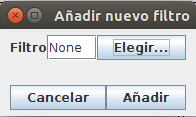
\includegraphics[width=0.4\textwidth]{img/anexo/Filtro_dialog1}
		\caption{Diálogo para la selección de filtro.}\label{fig:img/anexo/Filtro_dialog1}
	\end{figure}
%	\imagen{img/anexo/Filtro_dialog1}{Diálogo para la selección de filtro.}

	\begin{figure}[!h]
		\centering
		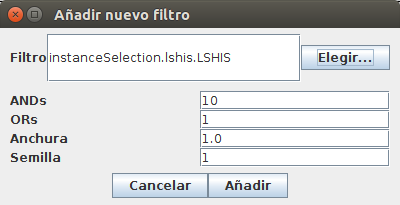
\includegraphics[width=0.6\textwidth]{img/anexo/Filtro_dialog2}
		\caption{Diálogo para la selección de filtro después de seleccionar un algoritmo.}\label{fig:img/anexo/Filtro_dialog2}
	\end{figure}		
\FloatBarrier						
%	\imagen{img/anexo/Filtro_dialog2}{Diálogo para la selección de filtro después de seleccionar un algoritmo.}
			
		\item \textbf{Panel de selección de clasificador y validación cruzada:} Su funcionalidad es similar a la descrita en paneles anteriores, concretamente el panel de selección de filtro. Sin embargo, es este caso solo es posible añadir un único clasificador (así como solo una única configuración de validación cruzada), por lo que las opciones que típicamente se mostraban en un diálogo separado, ahora se muestran en la propia pantalla (ver imagen \ref{fig:img/anexo/Clasificador_dialog}).
			
	\begin{figure}[!h]
		\centering
		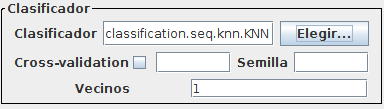
\includegraphics[width=0.8\textwidth]{img/anexo/Clasificador_dialog}
		\caption{Panel para la configuración del clasificador y la validación cruzada.}\label{fig:img/anexo/Clasificador_dialog}
	\end{figure}		
			
			
%	\imagen{img/anexo/Clasificador_dialog}{Panel para la configuración del clasificador y la validación cruzada.}			
			
		\end{itemize}
	\item \textbf{Menú inferior:} Cuenta con dos botones para ejecutar diferentes acciones. La modalidad ``ZIP'' será descrita en la subsección \ref{subsec:createZip}, pero en esta sección nos interesa presionar el botón ``Ejecutar''.
	\end{itemize}
	
Antes de lanzar una ejecución surge la pregunta de cuantas ejecuciones diferentes se han programado. Se generarán tantas ejecuciones como posibles combinaciones entre componentes se puedan crear con las configuraciones propuestas. Así pues, si, por ejemplo, se han indicado dos configuraciones de Spark, dos conjuntos de datos y dos filtros se realizarán $2 \times 2 \times 2 = 8$ ejecuciones, puesto que el clasificador será siempre el mismo.
	
Una vez hemos cumplimentado todos los campos requeridos (los únicos opcionales son los que se refieren a la validación cruzada) y presionamos sobre el botón ``Ejecutar'' veremos como en la esquina inferior izquierda se muestra un nuevo texto indicando la ejecución que se está realizando. Un ejemplo de un experimento completamente configurado y en funcionamiento puede verse en la imagen \ref{fig:img/anexo/Interfaz_completa_rellena}

\imagen{img/anexo/Interfaz_completa_rellena}{Ventana principal de la interfaz gráfica rellena.}

No se pueden lanzar varias baterías de experimentos a la vez, así que si intentásemos crear una nueva ejecución y ejecutarla mientras la anterior continúa funcionando recibiremos un mensaje de error.

Una vez terminadas todas las ejecuciones, la interfaz nos informará de ello mediante un nuevo diálogo. Podemos ir a consultar el resultado en el directorio \textit{results} que se ha generado en la carpeta desde la que hemos lanzado la ejecución. Si hemos iniciado el programa haciendo doble clic sobre el fichero .jar este directorio probablemente se encuentre en la carpeta \$HOME del usuario.

\subsection{Definición de una batería de ejecución y lanzamiento por separado}\label{subsec:createZip}

El procedimiento inicial es similar al marcado en el método de lanzamiento anterior, es decir, una vez abierta la interfaz gráfica hemos de indicar todas las configuraciones de ejecución que deseemos. La diferencia esta vez la encontramos al final de la operación, donde en lugar de presionar sobre el botón ``Ejecutar'', lo haremos sobre el botón ``ZIP''

Esta operación, que tal vez puede tardar unos instantes si hemos seleccionado conjuntos de datos muy grandes, generará una carpeta de nombre ``zip'' en el directorio desde donde hemos invocado la interfaz gráfica. Dentro de la carpeta encontraremos un nuevo archivo .zip que contendrá un script de ejecución .sh junto con todos los conjuntos de datos que necesitemos para realizar las ejecuciones que hemos definido previamente.

Ese fichero lo moveremos a donde sea necesario, típicamente un servicio clúster donde se encuentre Spark instalado junto con nuestra librería en el directorio \textit{\$SPARK\_HOME/lib}, tal y como se ha indicado en la sección destinada a la instalación de nuestra librería en \ref{subsec:InstalarISAlgorithms}.

Una vez allí, el archivo puede descomprimirse usando el comando: 

\begin{lstlisting}[language=bash]
$ unzip <fichero-zip>
\end{lstlisting}

Es posible que, para descomprimir el archivo necesitemos un paquete \textit{unzip} instalado. Si no existe, podremos obtenerlo con el comando

\begin{lstlisting}[language=bash]
$ sudo apt-get install unzip
\end{lstlisting}

Finalmente, hemos de ejecutar el archivo .sh que acabamos de descomprimir. Para ello, desde consola, podemos movernos a la ruta donde se encuentre el fichero y escribir en terminal:

\begin{lstlisting}[language=bash]
$ chmod +x Bateria_de_Ejecucion.sh
$ ./Bateria_de_Ejecucion.sh
\end{lstlisting}

Deberían comenzar las ejecuciones en Spark, una tras otra, hasta que finalicen todas.

\subsection{Lanzamiento en el servicio Google Cloud Dataproc}

Google Cloud Dataproc es uno de los muchos servicios que ofrece la plataforma Google Cloud (\url{https://cloud.google.com/}). Para acceder a todos ellos es necesario contar con una cuenta Google, cuyo proceso de registro no será descrito en este manual. Igualmente, existen diferentes maneras de utilizar este servicio. En este apartado se describirá únicamente la manera de uso gráfica, por ser la más intuitiva para realizar labores sencillas.

Lo primero que debemos saber es que los servicios ofrecidos en Google Cloud (incluido el propio Google Cloud Dataproc) suelen están asociados a un proyecto concreto, aunque, si acabamos de registrarnos, ya contaremos con un proyecto creado. De querer generar uno nuevo podemos hacerlo en el menú superior, clic sobre el nombre del proyecto actual y clic sobre ``Crear proyecto'' en el menú desplegable que generará la acción anterior (ver imagen \ref{fig:img/anexo/dataproc_crearProyecto}).

\imagen{img/anexo/dataproc_crearProyecto}{Creación de un nuevo proyecto en Google Cloud.}

Es importante indicar que, en el caso de estar realizando esta tarea con la versión de prueba de Google Cloud, no deberemos crear un nuevo proyecto, pues la condición gratuita se aplica solo al proyecto generado por defecto por Google.

Una vez tengamos nuestro proyecto nos encontraremos ante su página de inicio (ver imagen \ref{fig:img/anexo/dataproc_inicio}), aunque no entraremos a explicar el funcionamiento de la misma.

\imagen{img/anexo/dataproc_inicio}{Página de inicio de un proyecto en Google Cloud.}

El segundo paso será almacenar nuestro archivo .jar, junto con los conjuntos de datos, en algún lugar que Google pueda alcanzar. Para ello, lo más sencillo será usar un segundo servicio de Google Cloud: Google Cloud Storage. Podemos acceder a él desde el menú superior, haciendo clic sobre el icono situado más a la izquierda y seleccionando el servicio ``Storage'' de entre las opciones que muestre el menú emergente (ver imagen \ref{fig:img/anexo/dataproc_selectService}).

\imagen{img/anexo/dataproc_selectService}{Menú de selección de servicios de Google Cloud.}

Si el proyecto es nuevo, es posible que tengamos que reservar un nuevo segmento de memoria para poder guardar nuestros datos. Simplemente hacemos clic sobre la opción ``Crear segmento'' que veremos en el centro de nuestra pantalla y rellenamos los campos de ``Nombre'', ``Clase de almacenamiento'' y ``Ubicación'' acorde a nuestras preferencias. Una vez terminado este paso, podemos acceder a nuestro nuevo espacio de memoria y administrarlo según nuestro gusto mediante las opciones del menú superior o arrastrando hacia la ventana del navegador todos aquellos elementos que deseamos que sean subidos al servicio de almacenamiento.

Ahora, necesitar asignar ciertos permisos a nuestro proyecto para poder asignarle un clúster. Para ello, vamos a visitar el servicio ``Compute Engine'' de la misma manera que antes visitamos ``Storage'', presionando el icono de la izquierda en el menú superior y buscando el servicio entre la lista de posibles. Lo primero que se nos preguntará es si deseamos asignar una serie de permisos a nuestro proyecto, a lo cual aceptaremos.

Con todo preparado, vamos a acceder finalmente al servicio que realmente nos interesa: Google Cloud Dataproc. Repetimos la misma operación anterior y buscamos servicio ``Dataproc''.

Ahora, vamos a crear nuestro primer clúster. Presionamos sobre el botón ``Crear nueva agrupación'' que veremos en el centro de la pantalla y rellenamos el formulario que permitirá crear un clúster. Es importante saber que:

\begin{itemize}
\item Es conveniente situar la ubicación del clúster en la misma que el segmento de memoria que está destinado a usar.
\item Si estamos ejecutando desde la versión gratuita de Google Cloud, el tamaño del clúster estará limitado a 8 CPUs, incluyendo el nodo maestro.
\item En el apartado ``Opciones de acceso, inicialización, versión, red, segmento y trabajadores prioritarios'' podemos seleccionar la ``versión de imagen'' del clúster, lo que definirá la versión de los productos que vamos a usar. Este proyecto se ha probado con la versión 0.2 que incluye Spark 1.5.2
\item También en el apartado ``Opciones de acceso, inicialización, versión, red, segmento y trabajadores prioritarios'' hay una opción llamada ``Segmento de aplicación de fases de Cloud Storage''. Aquí debemos indicar el segmento de memoria que hemos creado anteriormente. Si no especificamos nada se creará uno por defecto.
\end{itemize}

\imagen{img/anexo/dataproc_clusterMenu}{Pantalla principal de Google Cloud Dataproc}

Bien, con nuestro clúster creado únicamente falta definir la tarea que debemos ejecutar.
Para ello, en el menú lateral izquierdo podremos ver una sección llamada ``Tareas'' (ver imagen \ref{fig:img/anexo/dataproc_clusterMenu}). Nos podemos dirigir a ella y crear una nueva tarea del mismo modo que hemos creado anteriormente un segmento de memoria o una agrupación. De nuevo, es importante tener en cuenta que:

\begin{itemize}
\item Deberemos definir el ``Tipo de tarea'' como ``Spark''
\item La ruta al archivo .jar (o al fichero que contenga el conjunto de datos cuando introduzcamos las opciones) tendrá una estructura similar a ``gs://nombreSegmento/directorio/fichero'' si hemos utilizado el servicio Google Cloud Dataproc.
\end{itemize}

Podemos ver un ejemplo de una configuración en la imagen \ref{fig:img/anexo/dataproc_tareaConfigurada}.

\imagen{img/anexo/dataproc_tareaConfigurada}{Ejemplo de una tarea configurada}

Lanzada la aplicación seremos redirigidos a una nueva pantalla donde podremos observar una línea de comandos tal y como si hubiésemos  lanzado la aplicación en nuestra propia máquina. Mientras la ejecución tiene lugar podemos realizar cualquier otro tipo de operación, incluido definir nuevas tareas.

Una vez terminada la tarea que hayamos programado, queda ver el fichero resultante de la aplicación, para lo que deberemos conectarnos al nodo maestro. Accedemos a la vista principal de nuestro clúster desde la pantalla principal de Google Dataproc (ver imagen \ref{fig:img/anexo/dataproc_clusterMenu}) y allí hacemos click sobre ``Instancias de VM'' y sobre el botón ``SSH'' que aparecerá junto al nombre del nodo maestro.
Esto abrirá una nueva ventana del navegador que emulará una consola de comandos. No es objetivo de esta sección hablar de todas las posibles opciones que podemos realizar, únicamente veremos el fichero resultante ejecutando el siguiente comando:

\begin{lstlisting}[language=bash]
$ cat /tmp/nombre_tarea/results/nombre_fichero_resultados
\end{lstlisting}

\subsection{Cheatsheet}\label{subsec:cheatsheet}
A continuación se va realizar un listado con todas las posibles opciones que actualmente pueden formar parte de la sentencia de invocación del programa.

 \begin{table}
  \begin{center}
   \begin{tabular}{| m{3cm} | L{9cm} |}
    \hline
    \centering Parámetro &  Descripción \\
    \hline
    \rowcolor{gray}
    \multicolumn{2}{|m{13cm}|}{\centering Tipo de ejecución} \\
    \hline
   	\centering ISClassExec & Define una tarea en la que intervenga un algoritmo de selección de instancias y un clasificador \\
   	\hline
   	\centering ISClassExecTest & Define una tarea en la que intervenga un algoritmo de selección de instancias y un clasificador y, además mide el tiempo de ejecución de la labor de filtrado.\\
   	\hline
   	\rowcolor{gray}
   	\multicolumn{2}{|m{13cm}|}{\centering Parámetros del lector} \\
   	\hline
   	\centering -f & Indica que el atributo de clase es el primero de los atributos de cada instancia.\\
   	\hline
   	\centering -hl + Int & Indica que existe una cabecera en el fichero y cuantas líneas forman dicha cabecera. \\
   	\hline
   	   	\rowcolor{gray}
   	\multicolumn{2}{|m{13cm}|}{\centering Parámetros para el selector de instancias} \\
   	\hline
   	   	\rowcolor{lightgray}
   	\multicolumn{2}{|m{13cm}|}{\centering instanceSelection.lshis.LSHIS} \\
   	\hline
   	\centering -and + Int & Número de funciones AND.\\
   	\hline
   	\centering -or + Int & Número de funciones OR.\\
   	\hline
   	\centering -w + Double & Anchura de los \textit{buckets}.\\
   	\hline
   	\centering -s + Long & Semilla utilizada para generar números aleatorios.\\
   	\hline
   	\rowcolor{lightgray}
   	\multicolumn{2}{|m{13cm}|}{\centering instanceSelection.demoIS.DemoIS} \\
   	\hline
   	\centering -rep + Int & Número de votaciones a realizar.\\
   	\hline
   	\centering -alpha +  Double & Valor alpha.\\
   	\hline
   	\centering -np +  Int & Número de particiones en las que se dividirá el conjunto de datos original. \\
   	\hline
   	\centering -dsperc + Double & Porcentaje del conjunto de datos utilizado para calcular el error durante el cómputo del fitness. \\
   	\hline
   	\centering -s + Long & Semilla utilizada para generar números aleatorios.\\
   	\hline
   	   	\rowcolor{gray}
   	\multicolumn{2}{|m{13cm}|}{\centering Parámetros para el clasificador} \\
   	\hline
   	   	\rowcolor{lightgray}
   	\multicolumn{2}{|m{13cm}|}{\centering classification.seq.knn.KNN} \\
   	\hline
   	\centering -k + Int & Número de vecinos más cercanos\\
   	\hline

   \end{tabular}
   \caption{Cheatsheet}
   \label{tabla:cheatsheet}
  \end{center}
 \end{table}



\bibliographystyle{plain}
\bibliography{bibliografiaAnexos}

\end{document}